\documentclass[twocolumn]{svjour3}
    

\usepackage{graphicx}      % include this line if your document contains figures
\usepackage{natbib}        % required for bibliography
\usepackage{enumerate}
\usepackage[utf8]{inputenc}
%\usepackage{float}
%\usepackage[centerlast,small,sc]{caption} 
%\setlength{\captionmargin}{30pt}
%\usepackage[none]{hyphenat} 
%\usepackage{subcaption} 
%\usepackage{capt-of}
%\usepackage{kpfonts}
%\usepackage{calc}
\newlength\shlength
\newcommand\xshlongvec[2][0]{\setlength\shlength{#1pt}%
  \stackengine{-5.6pt}{$#2$}{\smash{$\kern\shlength%
    \stackengine{7.55pt}{$\mathchar"017E$}%
      {\rule{\widthof{$#2$}}{.57pt}\kern.4pt}{O}{r}{F}{F}{L}\kern-\shlength$}}%
      {O}{c}{F}{T}{S}}
%\sloppy  
\journalname{Journal of Control, Automation and Electrical Systems}
\begin{document}

%\begin{frontmatter}

\title{State of the art and conceptual design of robotic solutions for
\textit{in situ} hard coating of hydraulic turbines}%\thanksref{footnoteinfo}} 



\author{Renan S. Freitas \and
		Gabriel Alcantara C. S. \and
		Eduardo Elael M. S. \and
		Estevão Fróes \and
		Ramon R. Costa}

\institute{Department of Electrical Engineering, COPPE
UFRJ, Rio de Janeiro, Brasil.
\email{renan028@gmail.com}}

\thanks{This work is supported by ESBR under contract COPPETEC
JIRAU 09/15 6631-0003/2015 (ANEEL R\&D program).}

\maketitle
  
\begin{abstract}      
Hydropower turbine's blades demand regular maintenance for flow stability and
turbine efficiency as they are constantly exposed to abrasion and cavitation
phenomena. Hard coating techniques by thermal aspersion are used to reduce the
erosion of the turbine's blade, thus increasing its life cycle, and to increase
turbine efficiency. Currently, applying a new coating layer requires turbine
disassembling, and recalibration. EMMA is an R\&D project of a robotic system
to perform hard coating by thermal spray on hydraulic turbine blades within the
turbine environment, i.e., hard coating application to an installed blade,
significantly reducing the downtime for hard coating process.
This document makes a survey of the state of the art of \textit{in situ}
turbine systems, and describes the conceptual designs for EMMA's robot and its
mechanical bases. The results outlines the next steps for EMMA and future
projects in the same area.

\keywords{hard coating \and hydropower \and turbine \and thermal spray \and
robotics \and in situ}
\end{abstract} 

\section{Introduction}
According to the world energy council, hydropower is the most flexible and
consistent of the renewable energy resources and, at the end of 2008, the total
capacity of hydropower resources was 874 GW. Brazil is the second
country in hydropower production, and second with the highest
consumption of hydropower with a 70.000 MW installed capacity, and 433
hydroelectric plants in operation. Since Brazil is one of the world's richest
countries in water resources, and the hydropower is the most dominant across
the country, it motivates the development and investment in hydropower
generation.
%\begin{figure}[h!]
%	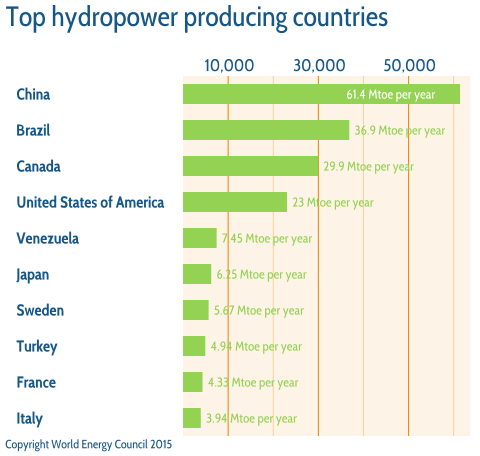
\includegraphics[width=\columnwidth]{figs/intro/graph.png}
%	\caption{Top hydropower producing countries}
%	\label{fig::cavitacao}
%\end{figure}

%O Brasil é um dos países mais ricos do mundo em recursos hídricos, facilitando
% o desenvolvimento e investimento em geração de energia a partir desse recurso. A
%energia hidráulica é a mais dominante em todo o país, e o Brasil é o segundo
%país com maior consumo de energia hidrelétrica no mundo com capacidade
%instalada de 70.000 MW, 433 usinas hidrelétricas em operação. 

In Brazil, the renovation and improvement of the built large plants is estimated
to result in a potential increase of 32.000 MW \citep{goldemberg2007energia}, a
figure that can be achieved, in large part, by the maintenance of the
hydropower turbines. These turbines are constantly exposed to abrasion and
cavitation phenomena, which determine its life cycle.
%Estima-se que a reforma e melhoria das grandes usinas construídas resultariam
%em um aumento potencial de 32.000 MW \citep{goldemberg2007energia},
%número que pode ser alcançado, em grande parte, pela manutenção das turbinas
%geradoras da energia elétrica. As turbinas estão constantemente expostas aos
%fenômenos de abrasão e cavitação, os quais determinam sua vida útil.

The cavitation phenomenon is very well studied and detailed in
\cite{escaler2006detection}, which outlines their types, occurrences and
effects in the different hydraulic turbines. This physical phenomenon can cause
erosions in the hydraulic turbines, leading to water flow instability,
excessive vibrations and turbine efficiency reduction.
%O fenômeno de cavitação está muito bem estudado e detalhado em
%\cite{escaler2006detection}, onde são apresentadas seus tipos, ocorrências e os
%efeitos nas diferentes turbinas. Esse fenômeno físico pode causar erosões na
%máquina hidráulica (figura~\ref{fig::cavitacao}), gerando instabilidade de
% fluxo de água, vibrações excessivas e redução da eficiência da turbina.

\begin{figure}[h!]	
	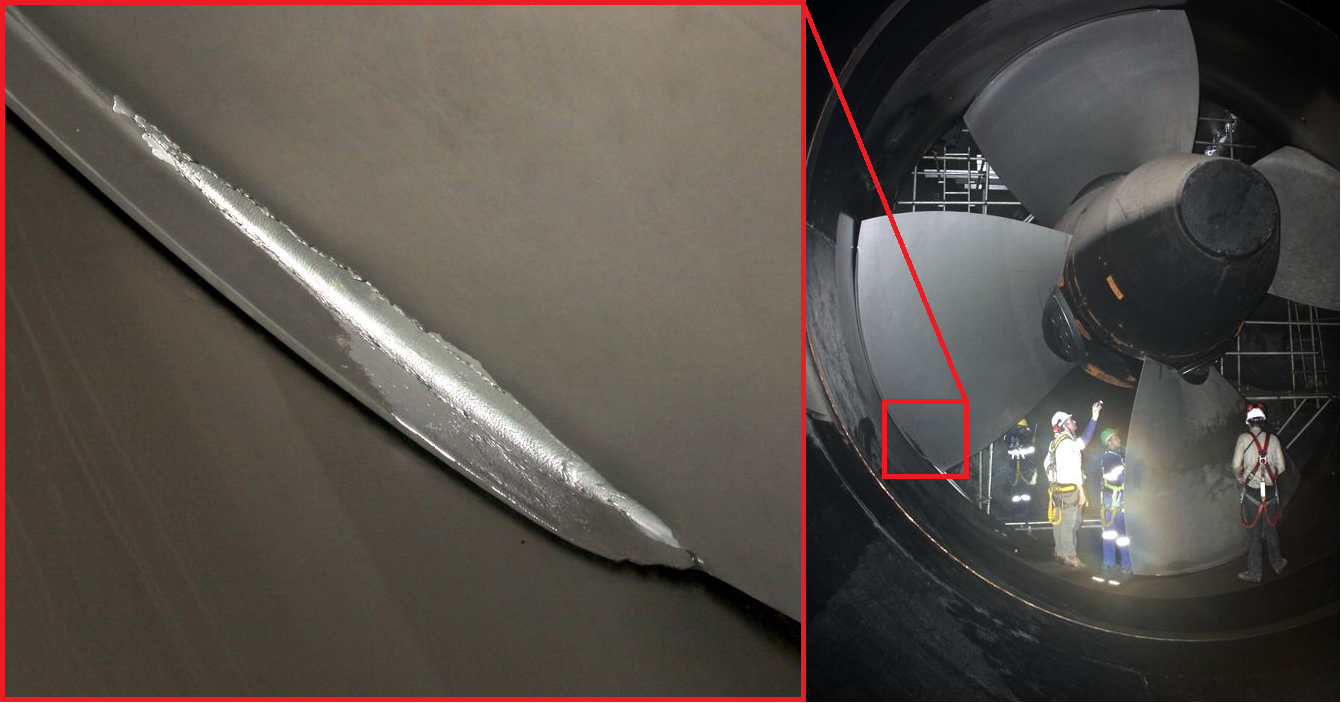
\includegraphics[width=\columnwidth]{figs/intro/cavitacao2.png}
	\caption{Jirau hydraulic turbine's blade eroded by cavitation.}
	\label{fig::cavitacao}
\end{figure}

Hard coating techniques by thermal aspersion
are used to reduce the erosion of the turbine's blade from cavitation or
abrasion, thus increasing its life cycle. This solution is analogous to a paint
that protects walls from environment exposure. The hard coating procedure is performed
before the hydraulic turbine installation by a robotic manipulator. The
procedure requires a robotic system due to high precision, speed, and
the hazardous substances that are used, as propane and other gases.
Although sufficient for blade protection, the coating also has a life
cycle itself, thus it needs to be redone from time to time to ensure the
blade's protection from physical phenomena.
%A fim de reduzir o desgaste da pá contra cavitação ou abrasão e aumentar a sua
%vida útil, utiliza-se a técnica de revestimento por asperção térmica, que pode
%% ser comparada com uma tinta que protege à exposição com o ambiente. O
% procedimento é realizado
%antes da instalação das pás na turbina por um robô, pois exige alta precisão
%e velocidade, além de expelir substâncias nocivas à saúde. Apesar de suficiente
% para a proteção da pá, o revestimento também tem vida útil e precisa ser refeito de tempos em tempos para
%garantir a proteção da pá contra os fenômenos físicos.

In the specific case of the Jirau hydroelectric dam, built on the Madeira
river, the number of suspended particles that the river carries intensifies the
abrasion phenomena, and Rijeza, a hard coating specialized company, identified cavitation erosion on blades, further reducing the coating life cycle.
Therefore, Jirau hydroelectric dam needs regular maintenance, which,
in the present situation, would require stoppage of the turbine, removing the
blades, positioning the blades for coating, coating application, turbine assembling, and recalibration. The downtime to perform all
maintenance can take up to two months, meaning a huge loss in power generation .
%No caso específico da usina hidrelétrica de Jirau, construída no rio Madeira,
%os fenômenos de abrasão são intensos devido ao grande número
%de partículas que o rio carrega diariamente, reduzindo ainda mais a vida útil
% do revestimento.
%Portanto, há a necessidade de manutenção regular, o que, na situação atual,
%exige paralização da máquina, desmontagem da turbina, posicionamento de cada pá
%na área designada ao revestimento, aplicação do revestimento, montagem da
%turbina e recalibração. O tempo de paralização para a realização de
%toda a manutenção pode levar de um a dois meses, significando uma grande perda
%na geração de energia. 

EMMA is an R\&D project by Fundação Coordenação de Projetos, Pesquisas e Estudos
Tecnológicos (COPPETEC), in partnership with Rijeza company, Agência Nacional de
Energia Elétrica (ANEEL) and Energia Sustentável do Brasil (ESBR). Its first
stage is a technical feasibility study of a robotic system to perform
coating by thermal spray on hydraulic turbine blades within the turbine
environment. The project aims to significantly reduce the downtime for hard
coating process.
%A primeira etapa do projeto EMMA, pesquisa e desenvolvimento
%realizados pela Fundação COPPETEC, em parceria com a empresa Rijeza, ANEEL e
%ESBR, é um estudo de viabilidade técnica de um sistema robótico para realizar
%revestimento por aspersão térmica de turbinas \textit{in situ}, ou seja, dentro
%do ambiente da turbina (aro câmara). O projeto tem como objetivo reduzir
%significativamente o tempo de manutenção do revestimento por ser realizado no
%ambiente confinado da turbina e, portanto, não havendo necessidade de sua
%desmontagem.

This document is divided as follows: section 2 describes, in detail, the
problem, contextualizes the reader in the Jirau environment and
describes the robot's tasks; section 3 surveys the state of the
art; section 4 describes the conceptual designs for the robot and mechanical
bases; finally, the section 5 concludes and outlines the next steps for the
EMMA project.
%Este documento está dividido da seguinte forma: a seção 2 descreve
%detalhadamente o problema, contextualiza o leitor no ambiente da usina de
%Jirau e descreve as possíveis tarefas do robô; a seção 3 faz um levantamento do
%estado da arte; a seção 4 descreve os projetos conceituais para o robô; e a
%seção 5 conclui e descreve os próximos passos para o projeto EMMA. 
 
\section{The problem}\label{sec::consideracoes}

Cavitation and abrasion in hydropower turbines cause surface erosion and
blade's hydraulic profile deformation, resulting in efficiency
reduction. A preventive solution is the High Velocity Oxygen Fuel (HVOF) coating
process of the blades. The hard coating creates a more lamellar structure,
increasing power generation efficiency, and provides greater
resistance to erosion. In the case of the Jirau hydroelectric dam, the coating
of turbine's blades is performed before turbine assembling and
installation. However, the abrasion due to a large number
of particles and sediment in the Madeira river, and the recent identified
cavitation require recoating in short intervals \citep{santa2009slurry}. Turbine
disassembling, recoating and turbine reassembling are very expensive process
and should be done regularly.

%O fenômeno de cavitação e abrasão em hidroturbinas provoca desgaste
%superficial por erosão e alteração do perfil
%hidráulico da pá, gerando redução da eficiência na geração de energia.
%Uma solução preventiva é o revestimento por metalização das pás, o qual aumenta
% a eficiência na geração de energia por gerar uma estrutura mais lamelar, e fornece maior
%resistência a desgastes. No caso da usina hidrelétrica de Jirau, o revestimento
%das pás é realizado antes da montagem e instalação da turbina, porém devido ao
% grande número de partículas e sedimentos que o rio madeira carrega e à cavitação, o revestimento
%deve ser aplicado novamente em intervalos curtos de tempo
%\citep{santa2009slurry}. A desmontagem da turbina, aplicação de novo
%revestimento nas pás e remontagem são um processo muito custoso e deverá ser
%feito regularmente. Portanto, há a necessidade de o procedimento ser
%executado dentro do aro câmara, \textit{in situ}, onde as pás são instaladas.

Cavitation is the formation of vapor cavities (bubbles) in a liquid due to
sudden pressure drops. When the liquid is subjected to increased pressure,
the bubbles implode, causing shock waves \citep{brennen2013cavitation}. 
In hydropower turbines, the cavitation occurs near the blades or
in the turbine output.% The liquid has the combination of kinetic components,
%gravitational potential, and energy flow. The kinetic component is due to the
%water flow (velocity), the potential depends on the altitude of the liquid, and
%the energy flow is the energy that a fluid contains due to pressure. According
%to the Bernoulli principle, the conservation of fluids, it implies that for
%the same altitude, increased kinetic component causes a reduction in pressure,
%occurring cavitation. 
The formation of large bubbles modifies the
characteristics of the flow , causing oscillations or vibrations on the
hydropower turbine, and negative affects the performance of the hydraulic
system. On the other hand, the collapse of small bubbles generates high
frequency shock waves, causing erosions on metal surface.
%A cavitação é a formação de cavidades de vapor (bolhas), em um líquido, devido
% a quedas repentinas de pressão. Quando o líquido é sujeito ao aumento de pressão,
%as bolhas implodem, ocasionando ondas de choque \citep{brennen2013cavitation}.
%Em hidroturbinas, o fenômeno de cavitação é comum próximo às pás ou
%na saída da turbina. O líquido apresenta a combinação
%de componentes cinético, potencial gravitacional e energia de fluxo. O
%componente cinético é em virtude do fluxo da água (velocidade), o potencial tem
%relação com a altitude, e a energia de fluxo é energia que um fluido contém
%devido à pressão que possui. De acordo com o princípio de Bernoulli, o
% princípio da conservação para os fluidos, implica-se que, para uma mesma altitude, o
%aumento da componente cinética acarreta em uma diminuição da pressão, ocorrendo
%cavitação. 
%Quando há cavitação, a formação de bolhas grandes altera as características do
%escoamento, ocasionando oscilações ou vibrações na máquina que, por
%conseqüência, prejudicam o rendimento do sistema hidráulico. As bolhas
%pequenas, ao colapsar, geram ondas de choque de alta frequência, podendo
% provocar erosões se próximo à superfície metálica.

%Além da cavitação, como a água atravessa o aro câmara em grande velocidade, o
%acúmulo de sedimentos irá provocar desgaste abrasivo, isto é, perda de material
%pela passagem de párticulas rígidas. 

In this section, the coating technology is addressed as the way to
reduce the damage by cavitation. Also, the reader is contextualized in
the Jirau hydroelectric plant problem. Finally,  robotic tasks are highlighted to
solve the problem.
%Nesta seção, são apresentadas as formas de reduzir os danos da cavitação pela
%tecnologia de revestimento por metalização, a contextualização do problema no
%caso da usina hidrelétrica de Jirau e as tarefas que um sistema robótico deve
%realizar para solucionar o problema.


\subsection{The HVOF coating process}\label{sec::desc_hvof}
The thermal spraying (or metallizing) is a process in which
heated materials are sprayed onto a surface in order to improve or
restore their properties and dimensions. The coating significantly increases the
resistance to erosion or corrosion.
%The different types of thermal spraying are: plasma spraying, detonation
%spraying, wire arc spraying, flame spraying, High velocity oxy-fuel coating
%spraying (HVOF), warm spraying and cold spraying.

%O revestimento por aspersão térmica (ou metalização) é um processo em que
%partículas aquecidas são pulverizadas em uma superfície a fim de melhorar ou
%restaurar suas propriedades e dimensões. O revestimento estende a vida útil do
%material, aumentando significantemente a sua resistência à erosão e corrosão.
%Os diferentes tipos de metalização são: por chama, arco elétrico, detonação,
%chama de alta velocidade (HVOF), plasma, a frio e a quente.

A thermal spraying system comprises: a spray gun, which partially melts and
accelerates the particles to be deposited onto metal surface; a feeder, which
provides the powder (particles) via pipes; a provi\-der of burning material; a robot (manipulator) to handle the gun; an
electric power supply to the gun; and a control console for the system.
%Um sistema de metalização é composto por: uma pistola de aspersão, responsável
%pelo derretimento e aceleração das partículas a serem depositadas na
%superfície; um alimentador, que fornece o pó (partículas) através de tubos;
%um fornecedor do material de combustão; um robô para manipular a pistola; uma
%fonte de alimentação elétrica para a pistola; um console de controle para o
%sistema.

In the specific case of Jirau, turbine blades (stainless steel 420) %,
%the thermal spraying type is HVOF on both sides of the blade, and executed 
are coated on High Velocity Oxy-Fuel (HVOF) thermal spraying type by the
Rijeza company with a robotic manipulator 150 kg payload, which is a good
safety margin, since the system mass is 10 kg (cables and gun). The process
takes 6 hours per side of the blade.
%No caso específico das pás (aço inox 420) das turbinas da usina hidrelétrica de
%Jirau, antes da montagem da turbina, a metalização tipo HVOF é realizada em
%ambos os lados da pá pela empresa Rijeza com um manipulador industrial de 150
% kg de carga máxima, permitindo controle de vibrações com boa margem de segurança, já que a massa do
%sistema pode chegar a 10 kg (cabos e pistola). O tempo
%mínimo do processo é de 6 horas por lado da pá.

The HVOF consists of feeding, in a combustion chamber, the coating material
(tungsten carbide), a gaseous fuel mixture (propane), and oxygen. According to
the data provided by the Rijeza company, the 8 kg spray gun projects a flame of
$3000^\circ$C, spraying the particles at 700 to 1000 m/s speed, and
generating a 15 N recoil force.
%O HVOF consiste em alimentar, numa câmara de combustão, o material de
%revestimento (carboneto de tungstênio), uma mistura gasosa do combustível
% (propano) e oxigênio. De acordo com os dados fornecidos pela empresa Rijeza, a pistola de 8
%Kg projeta uma chama de $3000^oC$, que pulveriza as partículas com velocidade
% de 700 a 1000 m/s, gerando uma força de recuo de 15 N.

The manipulator must have 5 mm accuracy, and the spray gun should remain
at a 210 to 240 mm distance with $90^\circ\pm 60^\circ$ angle in respect to the metallic
surface plane for a regular coating layer. The end effector of the manipulator
must control the spray gun at a constant 40 m/min speed, and should not stop during the process with
the blade in its range (\textit{long stop}), otherwise coating material would
accumulate.
The end effector direction changes are considered \textit{long stop} too, thus
direction changes should be made out of the blade range, or sacrifice plates
should be used. Sacrifice plates, or masking, are metal plates placed on blade
spots that should not be coated. 
%O manipulador robótico deve possuir precisão de 5 mm, a pistola no efetuador
%deve permanecer a uma distância que varia entre 230 e 240 mm, e ângulo de $90^o
%\pm 60^o$, em relação à superfície. O manipulador deve ser capaz de
%mover a pistola a velocidade constante de 40 m/min, e não pode permanecer uma
%posição da pá por muito tempo (parada), pois há acúmulo de material, deformando
% a superfície. Trocas de direção ou sentido na movimentação do manipulador são
%considerados como parada, logo as trocas deverão ser realizadas em áreas
%exteriores à superfície da pá ou chapas de sacrifício são utilizadas. 
%Placas de sacrifício, ou mascaramento, são chapas colocadas em regões onde as
%peça não podem ser jateadas ou revestidas. Geralmente uma chapa de qualquer
% tipo de aço pode ser utilizada, pois a chama não fica parada sobre ela por um longo
%período, não aquecendo-a o suficiente para danificar. Quando a pistola
%permanece, em funcionamento, a chama é apontada para algum lugar onde não tenha
% obstáculos.

 % As informações do processo
% podem ser observadas na figura~\ref{fig::hvof}.
 
%\begin{figure}[h!]	
%	\includegraphics[width=\columnwidth]{figs/intro/hvof.pdf}
%	\caption{Foto do efetuador do manipulador e pistola HVOF.}
%	\label{fig::hvof}
%\end{figure}

Regarding the operating conditions, the hydropower turbine is a confined
space, the HVOF process has excessive audible noise (100-140 dB), and hazardous
and potentially explosive gases are expelled; the blade can reach up to
$110^\circ$C; the environment's temperature and humidity should be monitored and
ideally set for the coating process; and $40\%$ of the sprayed particles are
lost during the process \citep{wu2006rebound}, which are spread throughout
the environment. Thus, the process requires a very well
ventilated environment. Table~\ref{tab::hvof} summarizes the project
restrictions and specifications.
%Em relação às condições de operação: o espaço da aplicação HVOF é confinado,
%com excesso (100 a 140 dB), gases nocivos e com risco de explosão podem
%ser exalados; a pá pode atingir temperaturas de até $110^oC$; as condições de
%umidade e temperatura devem ser ideais para o processo; e há perda de $40\%$
%das partículas pulverizadas  \citep{wu2006rebound}, que são espalhadas pelo
%ambiente. Portanto, algumas medidas devem ser tomadas para a execução do
%processo: a operação deve ser remota, não há presença de pessoas \textit{in
%loco}; os gases presentes e umidade/temperatura devem ser constantemente
%monitorados; o robô manipulador é selado; as partículas desperdiçadas devem
%ser removidas (limpeza); e o desligamento do sistema deve ser acompanhado por
% corte de gás.

%Finally, the coating quality is evaluated by an instrument which measures
%surface porosity, oxidation , hardness and roughness. The measurement is
%performed manually, quickly and easily by an operator.
%A qualidade do revestimento é geralmente avaliada por um instrumento que
%realiza a medida de porosidade, oxidação, dureza e rugosidade da superfície. O
%processo é realizado manualmente, de maneira rápida e fácil, por um operador.

%A tabela~\ref{tab::hvof} resume as restrições e especificações do
%projeto:

\begin{table}
% table caption is above the table
\caption{HVOF process data}
\label{tab::hvof}

\begin{tabular}{ll}
\hline\noalign{\smallskip}
Component & Data \\
\noalign{\smallskip}\hline\noalign{\smallskip}
Spray gun mass & 8 Kg  \\
Cables mass & 12 Kg  \\
Flame temperature & $3000^\circ$C \\
Spray gun recoil & 15 N \\
Manipulator precision & 5 mm \\
Spray gun to blade distance & 230-240 mm \\
Spray gun to blade angle & $30^\circ$-$90^\circ$ \\
Manipulator velocity & 40 m/min \\
HVOF sound noise & 100 a 140 dB \\ 
Blade temperature & up to $110^\circ$C \\
\noalign{\smallskip}\hline
\end{tabular}
\end{table}

%\begin{center}
%\begin{tabular}{  c | c  }
%  \hline
%  \textbf{Componente} & \textbf{Dado} \\ \hline
%  Massa da pistola HVOF & 8 Kg  \\ \hline
%  Massa dos cabos HVOF & 12 Kg  \\ \hline
%  Tempo HVOF por pá & 6 horas \\ \hline
%  Temperatura da chama HVOF & $3000^oC$ \\ \hline
%  Recuo da pistola & 15 N \\ \hline
%  Precisão do manipulador & 5 mm \\ \hline
%  Distância pistola-pá & 230-240 mm \\ \hline
%  Ângulo pistola-pá & $30^o$-$90^o$ \\ \hline
%  Velocidade do manipulador & 40 m/s \\ \hline
%  Ruído HVOF & 100 a 140 dB \\ \hline
%  Temperatura da pá & $110^oC$ \\
%  \hline
%\end{tabular}
%\captionof{table}{Dados principais do processo HVOF}
%\caption{Dados principais do processo de metalização HVOF}
%\label{tab::hvof}
%\end{center}

%Sistemas robóticos não devem utilizar magnetismo como meio de aderência, já que
%o aço inox 420 não apresenta alta permeabilidade magnética e a alta temperatura
%da pá deve inviabilizar essa solução. Adesão por ventosas é uma solução
%viável, pois material não causa dano ao revestimento, porém a escolha do
%material da ventosa deve ser estudado,já que a pá quente pode ocasionar em
%perda de sucção, como em ventosas emborrachadas.


\subsection{Requirements for HVOF process}

The HVOF process in hydropower turbines has some prerequisites for correct
coating application. This subsection details the appropriate blades surfaces
preparation to ensure the maintenance of the hydraulic profile.
%O processo de metalização de turbinas hidrelétricas tem alguns pré-requisitos
%que devem ser respeitados para uma correta aplicação e fixação da camada de
%material durante o revestimento. Essa subseção descreverá as etapas necessárias
%de preparação da superfície a fim de se assegurar a manutenção da qualidade dos
% resultados e do perfil hidráulico da pá. 

\subsubsection{Sandblasting}

According to Rijeza studies, recoating an already coating surface by
superimposition does not produce satisfactory results if compared the process
performed on a raw surface. Thus, it is recommended a abrasive blasting
operation to smooth the surface and remove the remaining coating.
%O processo de metalização sobreposto a uma superfície que já possui uma camada
%protetora desgastada não apresenta um resultado tão satisfatório se comparado
%com o processo realizado em uma superfície crua. Por esse motivo é recomendado
%que seja realizado um processo de jateamento abrasivo. 

Sandblasting consists in forcibly propelling a stream of abrasive material
against a surface under high pressure. The erosion creates an uniform
superficial layer. The sandblasting increases the surface roughness and
adhesion.
%O jateamento consiste em direcionar um fluxo de material abrasivo na superfície
%do material a fim de se erodir a mesma e retirar o material depositado na
% camada superficial. Outra característica desse processo é a capacidade de aumentar a
%rugosidade da superfície e, assim, aumentar o poder de adesão da nova camada a
%ser metalizada.  

In the specific case of turbine blades, the sandblasting process utilizes
aluminum oxide as abrasive material. An operator performs the sandblasting with
specialized equipment, which is composed a compressed air, and particles
of the abrasive jet.
%O processo de jateamento para o tratamento específico da superfície das pás da
%turbina utiliza óxido de alumínio como material abrasivo e pode ser realizado
%por um operador. A infraestrutura necessária para esse processo é uma fonte de
%ar comprimido, geralmente proveniente de um compressor de ar, para propulsionar
%o particulado que forma o jato abrasivo. %\textbf{A preparação do ambiente no
% envolto da pá, o escoamento do material e
%as consequências da realização desse processo não foram analisados} e,
%possivelmente, será necessária a implementação de infraestrutura de suporte
%para proteção dos equipamentos adjacentes que não receberão o jateamento,
%limpeza do material depositado e exaustão do particulado suspenso.

\subsubsection{Repare}

Damages on the blade surface can reduce its efficiency and even its integrity,
committing operation safety. The HVOF process can not repair severe surface
damage or structural damage, such as cracks. Therefore, blade inspection should
be performed before HVOF process, since the sandblasted surface facilitates
damage visualization.
%Danos existentes na superfície da pá ou em sua estrutura podem reduzir a sua
%eficiência e até mesmo a própria integridade da pá, prejudicando a segurança 
%da operação. O processo de metalização não tem a capacidade de reparar
%danos severos na superfície ou danos estruturais como rachaduras. A inspeção
%para procura desses defeitos deve ser realizada antes da realização do processo
%de metalização, uma vez que a superfície jateada, ou seja, em metal cru sem
%camada de proteção, facilita a visualização de danos. %Os procedimentos para
%reparos de danos estruturais ou referentes a rachaduras não serão cobertos por
%este documento.

The damages caused by cavitation, as explained in
section~\ref{sec::consideracoes}, modifies the blade hydraulic profile and
should be repaired. The repair procedure varies according to the severity of
the damage. Common repair procedures are:
%Os danos causado por cavitação, como explicado na seção
%\ref{sec::consideracoes}, pode alterar o perfil hidráulico da pá e deve ser
%reparado sempre que possível. O procedimento de reparo varia de acordo com a
%severidade dos danos causados. À medida que a profundidade das cavidades
% geradas na pá e a extensão dos danos vão aumentando, medidas mais extremas se tornam
%necessárias e, por isso, a estratégia de reparo para esse tipo de dano deve
%estar alinhada com o tipo de processo que se deseja utilizar. Inspeções e
%reparos mais frequentes significam processos mais simples, enquanto que reparos
%mais espaçados podem resultar até na inutilização da pá. Os procedimentos mais
%utilizados para o reparo de danos causados por cavitação são:

\begin{itemize}
  \item Non fused materials;
  \item Welding;
  \item Welding and solid plate.
\end{itemize}

\paragraph{Repair with non fused materials}

Minor damages are usually treated with non fused material processes, where it is
not necessary to fuse materials to fill the blade cavities. The processes and
materials used are: epoxy, ceramics, HVOF coating, neoprene and urethane.
%Para pequenos danos, é possível utilizar processos nos quais não é necessário
%fundir o material depositado para preenchimentos das cavidades ao material da
%superfície metálica da pá. Os processos e materiais utilizados, usualmente na
%indústria, são: 

%\begin{itemize}
%\item Epoxy;
%\item Cerâmica;
%\item Revestimento por metalização;
%\item Neoprene;
%\item Urethane.
%\end{itemize}

%Vale ressaltar que a solução proposta para a metalização de uma camada
% protetora para se evitar os danos causados pela cavitação também poderia ser utilizado
%para preencher danos passados, desde que respeitem o limite de espessura
%para o tipo de processo utilizado


\paragraph{Repair with welding}

Cavitation repair by welding is the most common procedure, as it allows high
material deposition and requires less maintenance. This process consists in
welding layers deposition. After the operation, the repairing surface should be
polished accordingly with the standard measures of quality for the blade
hydraulic profile. This procedure is usually performed manually by a highly
skilled operator. There are, also, in the literature, automated solutions, such
as the Scompi Robot and Roboturb \citep{roboturb,scompi}.
%O preenchimento dos danos causados devido à cavitação por solda é o
%procedimento mais comum, pois possibilita uma maior deposição de material e não
% obriga a realização de reparos com uma frequência elevada. Esse processo consiste na
%deposição de solda em camadas, até o completo preenchimento. A
%superfície deve ser, então, esmerilhada até entrar em conformidade com as
%medidas padrão de qualidade para o perfil hidráulico da pá a ser reparada. Essa
% tarefa é normalmente realizada por mão de obra altamente qualificada e existe, também,
%na literatura a presença de soluções automatizadas, como os robôs Roboturb e
% Scompi
%\citep{roboturb,scompi}

\paragraph{Repair by welding and solid plate}

Severe damages are usually repaired by solid plates, which would fill large
areas. The fixation process of the plates is carried out by welding, as well
as filling the remaining cavities. 
%Para casos de danos mais severos, pode ser necessária a utilização de placas
%para o preenchimento de grandes extensões. O processo de fixação das placas é
%realizado por solda, assim como o preenchimento do volume restante. O processo
%de solda, esmerilhamento e verificação é comum ao procedimento padrão
% utilizando somente solda.
















\subsection{Environment contextualization}\label{sec::desc_contex}

The Jirau plant has horizontal axis bulb type turbines. In hydropower
plants, electric power generation depends on the water level and river flow,
however bulb type turbines are designed just for high water flow to produce
enough electricity. The figure\ref{fig::bulb_turbine} and the
table\ref{tab::bulb_turbine} illustrate a bulb type turbine and the large
ducts needed to hold the large volume of water.
%A usina hidrelétrica de Jirau é do tipo fio d'água, na qual são utilizadas
% turbinas do tipo bulbo de eixo horizontal. Como a geração de energia depende da altura da queda d'água e da vazão do rio, as turbinas do tipo bulbo utilizam uma grande vazão de
%água para produzirem energia elétrica suficiente. A figura
%\ref{fig::bulb_turbine} e a tabela \ref{tab::bulb_turbine} ilustram uma turbina
%do tipo bulbo e o grandes dutos necessários para comportar o grande volume de
% água que passa através da turbina.
 
\begin{figure}[h!]	
	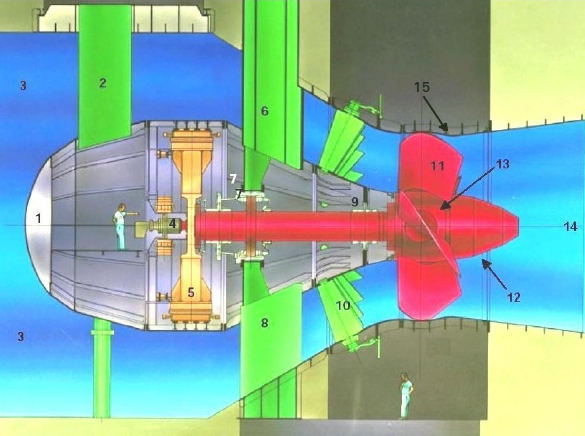
\includegraphics[width=\columnwidth]{figs/intro/bulb_turbine2}
	\caption{Bulb type turbine.}
	\label{fig::bulb_turbine}
\end{figure}

\begin{center}
\begin{tabular}{  c | c  }
  \hline
  \textbf{Número} & \textbf{Componente} \\ \hline
  1 & Nariz do bulbo \\ \hline
  2 & Tubo de acesso ao gerador  \\ \hline
  3 & Câmara de adução  \\ \hline
  4 & Cabeçote Kaplan  \\ \hline
  5 & Gerador Síncrono  \\ \hline
  6 e 8 & Estrutura de sustentação \\ \hline
  6 & Tubo de acesso à turbina \\ \hline
  7 e 9 & Mancais Combinado e Guia \\ \hline
  10 & Distribuidor \\ \hline
  11 & Pás do Rotor \\ \hline
  12 & Cone ou Ogiva \\ \hline
  13 & Cubo \\ \hline
  14 & Tubo de sucção/descarga \\ \hline
  15 & Aro Câmara \\
  \hline
\end{tabular}
\captionof{table}{Bulb type turbine principle components}
%\caption{Componentes principais de uma turbina tipo bulbo}
\label{tab::bulb_turbine}
\end{center}

Turbine repair or inspection requires water flow stoppage and water drainage. In
Jirau, there is a 80 cm diameter access (hatch) for rotor maintenance. In the
context of the proposed solution, the turbine points of interest are:

%Atualmente, caso seja necessário algum reparo ou inspeção na turbina, é
% necessário que se interrompa o fluxo de água e que toda a água em seu interior seja drenada. Para manutenção do rotor, existe uma escotilha de acesso de diâmetro limitado. Entretanto, caso deseje-se realizar 
%a metalização de pás já instaladas, utilizando-se os processos atuais, é
%necessária a retirada de todo o aro câmara, desmontagem completa do rotor e
% logística de transporte das pás até o local onde a metalização será realizada. Essa operação, caso necessite ser realizada, demandaria a mobilização
%de diversas equipes de manutenção, operação de pórtico rolante e transporte,
%além de impossibilitar a utilização da turbina durante várias semanas.
%No contexto da solução proposta, os pontos de interesse da turbina são:

\begin{itemize}
  \item propeller and blades;
  \item Ring chamber and adjacent areas;
  \item Hatcher of access;
  \item Suction tube;
  \item Available infrastructure.
\end{itemize} 

\subsubsection{Propeller and blades}
 
The rotor or turbine propeller consists of the hub, the blades and the cone.
Blades of Jirau turbine measure approximately 2.5 m tall and
3 m wide, they are fully reachable from the turbine interior,
excepting edges and lips, which can be visualized through a small top hatch
access. The figure\ref{fig::blade_rijeza} exemplifies a turbine blade recently
coated by Rijeza company. 
%O rotor ou hélice da turbina é constituído do cubo, as pás e o cone. 
%Nas turbinas da usina de Jirau, cada pá mede, aproximadamente, 2,5m de altura e
%3m de largura. A partir do interior da turbina, todas as superfícies da pá são
%alcançáveis, com exceção da borda e do lip da pá. O único ponto de acesso à
%essa regiâo é por meio da escotilha superior de acesso. A figura
%\ref{fig::blade_rijeza} exemplifica uma pá do rotor presente na usina de Jirau
% recém metalizada no galpão da Rijeza.

\begin{figure}[h!]	
	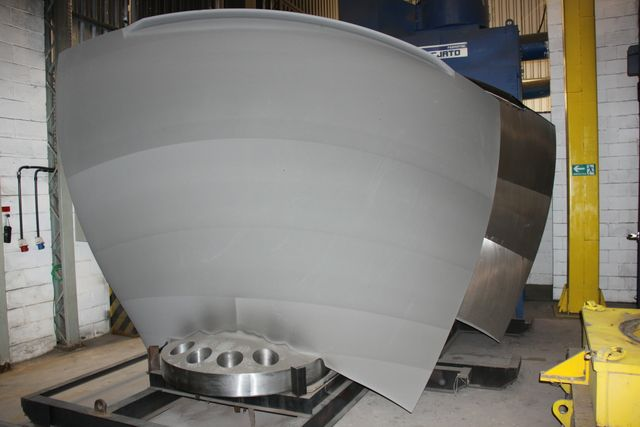
\includegraphics[width=\columnwidth]{figs/viagem/2015_04_28/Rijeza/img_4887}
	\caption{Jirau turbine blade.}
	\label{fig::blade_rijeza}
\end{figure}


The blades angles relative to the water flow can be changed $\pm 14.5$ from the
starting position, without overlapping areas, figure
\ref{fig::blades_angle}. These angles can be exploited to optimize working space
for blade coating process and also influences the working region between
the distributor and the rotor. Blades angles and rotor position can be changed
manually, and the last could be rotated in both directions without limit.
However, this operation is an imprecise and risky task. Hence, the proposed
solution should optimize rotations required for the blade processing.
%A angulação de cada pá em relação ao fluxo d'água pode ser alterado em 29$^o$,
%14.5$^o$ para cada lado a partir da posição inicial, não havendo sobreposição
%entre as pás, como ilustrado na figura \ref{fig::blades_angle}.
%Essa angulação pode ser explorada para otimizar o espaço de trabalho necessário
%para o processamento da pá e também influencia o acesso à região
%entre o distribuidor e o rotor, uma vez que não existe acesso pela montante da
%turbina. Entretanto, vale observar que esta angulação não pode ser alterada
%manualmente e só pode ser realizada uma vez, antes do desligamento da turbina.
% A posição do rotor também pode ser manualmente alterada, possibilitando que o
%mesmo seja girado em ambas as direções e sem limite de revoluções. Entretanto,
%essa operação é uma tarefa imprecisa e envolve um certo risco às pessoas que a
%realizam. Sendo assim, a solução proposta deve otimizar o número de rotações
%necessárias para o processamento de todas as pás.

\begin{figure}[h!]	
	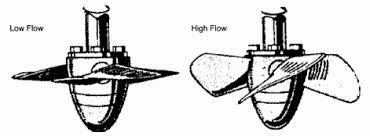
\includegraphics[width=\columnwidth]{figs/intro/blades_angle}
	\caption{Example of the blade angle limits.}
	\label{fig::blades_angle}
\end{figure}

\subsubsection{Ring chamber and adjacent regions}

The ring chamber, as the distributor area and the suction tube, has metal
surface. This characteristic allows magnetic fixing solutions for robotic
systems. However, the cylindrical and sloping shape of aro camara, and the
turbine distributor hinder robot fixation and movement. An horizontal plane or
an efficient and robust base should be build for the system fixation.
Under turbine maitenance, devices and equipments are fixed by scaffolding
anchored by ropes. The figure~\ref{fig::andaime} illustrates a turbine under
maintenance.
%O aro câmara, assim como o a região próxima ao distribuidor e também ao tubo de
%sucção possuem superfícies metálicas. Essa característica possibilita a
%exploração de soluções de fixação magnética.

%Somente a região compreendida pelo aro câmara é plana e tendo como agravante a
% presença do distribuidor na região à montante ao rotor. É necessário que a inclinação presente nessas superfícies seja contabilizada e uma solução eficiente 
%de apoio ou plano elevado seja desenvolvida caso haja necessidade de fixação de
% alguma parte do sistema. Atualmente todo o trabalho é realizado por meio da montagem de andaimes ancorados por cordas. A
%figura \ref{fig::andaime} ilustra uma estrutura utilizada no modo de inspeção e
%manutenção atuais.

\begin{figure}[h!]	
	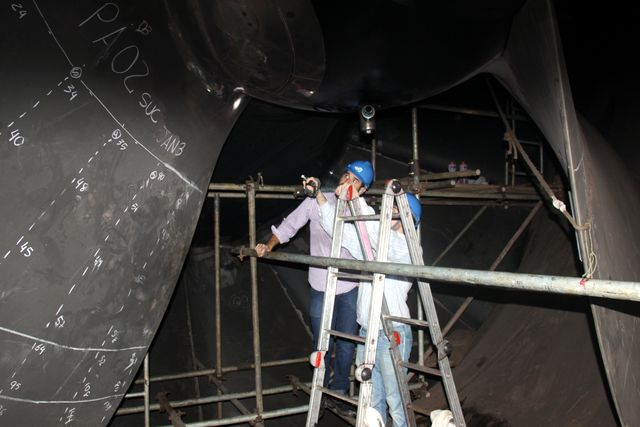
\includegraphics[width=\columnwidth]{figs/viagem/2015_04_28/UG/img_4969}
	\caption{Turbine under maintenance. Scaffolding as fixation points for
	equipments.}
	\label{fig::andaime}
\end{figure}

 
\subsubsection{Hatches}
The turbine accesses are two hatches: the bottom hatch is located at the
beginning of the suction tube, next to the ring chamber; and the top hatch is
located at the top of the ring chamber.
%O acesso à turbina se dá por duas escotilhas, uma inferior, localizada no
% ínicio do tubo de sucção próxima ao aro câmara e outra superior, localizada na parte superior do aro câmara.

Operators access the turbine via the bottom hatch and all equipments for
maintenance are transported through this hatch. The bottom hatch diameter is
80 cm.
%A escotilha inferior é o acesso utilizado para a entrada de pessoas na turbina
% e todo material utilizado para reparos é transportado através dessa escotilha. Na usina de Jirau existem dois 
%tipos de escotilha de acesso inferior, sendo a menor delas possuindo 80cm de
% diâmetro.

The top hatch is used mainly for blade lip visual condition inspection. The
diameter of the top access is approximately $35.7cm$, thus no equipments
are transported through this hatch. The figures~\ref{fig::esc_sup_ext} e
~\ref{fig::esc_sup_int} illustrate the top hatch from different views.
%A escotilha superior é utilizada, principalmente, para a inspeção visual do
%estado dos Lips das pás.
%O diâmetro do acesso superior é de aproximadamente $35.7cm$, limitando as
%dimensões dos equipamentos que podem ser transportados através da escotilha. As
% figuras \ref{fig::esc_sup_ext} e \ref{fig::esc_sup_int} ilustram o acesso à escotilha superior pelo exterior ao
%aro câmara e a visão pelo interior da turbina,
%respectivamente.

\begin{figure}[h!]	
	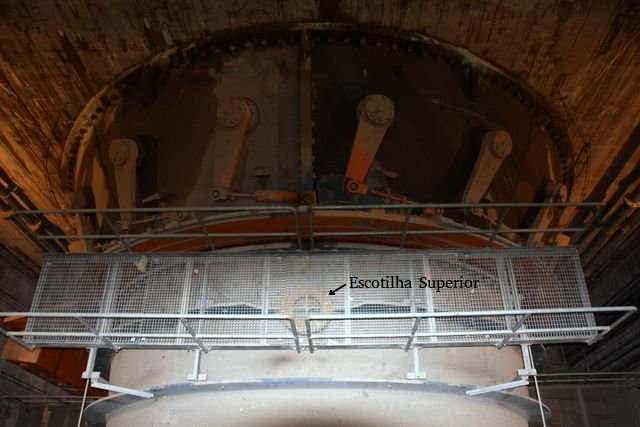
\includegraphics[width=\columnwidth]{figs/viagem/2015_04_28/UG/img_4979_mod}
	\caption{Top hatch view - ring chamber exterior}
	\label{fig::esc_sup_ext}
\end{figure}

\begin{figure}[h!]	
	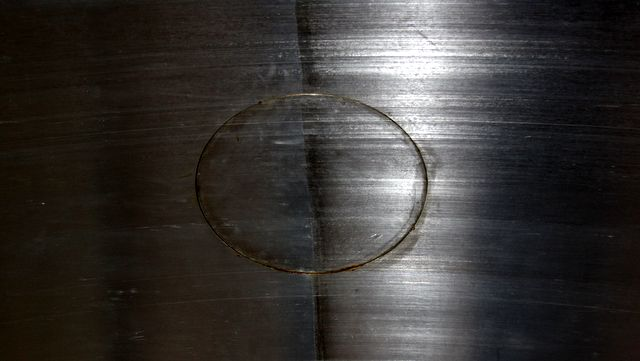
\includegraphics[width=\columnwidth]{figs/viagem/2015_04_28/UG/img_4982}
	\caption{Top hatch view - ring chamber interior}
	\label{fig::esc_sup_int}
\end{figure}

\subsubsection{Suction tube}

At the end of the discharge pipe is located the downstream stoplogs and then the
riverbed. If the stoplog are not inserted, there is a 10 m wide gap, which
could be used as access. However, the high water flow due to the
openning of the distributor make it impossible for access. The distributor is
not closed immediately due to environmental issues, since this becomes the
passage of fish.
%Ao final do tubo de descarga está localizado o vão dos stoplogs 
%de jusante ou da comporta vagão e, em seguida, o leito do rio. Caso os stoplogs 
%não estejam inseridos, existe um vão de, pelo menos, 10 m de largura. Porém,
% não é válida a utilização deste vão como acesso à turbina, pois há grande fluxo de
%água devido à abertura do distribuidor. O distribuidor não é fechado
%imediatamente por questões ambientais, já que este é o escoamento de peixes.

%criando assim
%um acesso extra para um sistema submarino. A figura \ref{fig::tubo_suc}
%exemplifica a magnitude do tamanho do acesso, deixando claro que o limitante de
%tamanho do sistema para a utilização desse acesso é o vão de entrada do
% stoplog, ilustrado na figura \ref{fig::stoplog}. Outra alternativa é utilizar um
%guindaste e submergir o sistema pelo próprio rio, entretanto o sistema ficaria
%sujeito as condições do ambiente.

\begin{figure}[H]	
	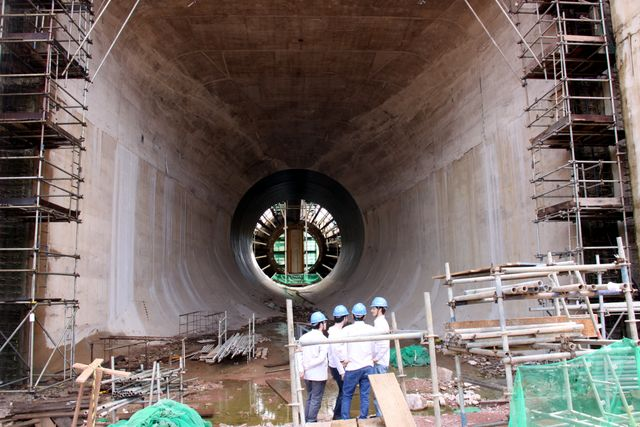
\includegraphics[width=\columnwidth]{figs/viagem/2015_04_30/Vao/img_5086}
	\caption{Suction tube openning under construction.}
	\label{fig::tubo_suc}
\end{figure}

\subsubsection{Available infrastructure}
After the turbine drainage, maintenance provides electricity and compressed
air, requirements for the HVOF process. Other important factor is the presence
of a gantry crane outside the turbine, but could position the HVOF necessary
equipment nearby the top hatch. Also, it is possible to access the top hatch
through the gantry crane.
%É importante ressaltar a infraestrutura dísponível para o desenvolvimento da
% solução.
%Após secar a turbina, é possível a disponibilização de energia elétrica e ar
%comprimo em seu interior, ambos importantes para o processo de metalização.
% Outro fator importante é a presença de um pórtico rolante que tem acesso até o andar diretamente 
%inferior ao aro câmara, posicionando todo o equipamento necessário nas
% proximidades da escotilha de acesso inferior. É possível também o acesso direto, por meio de pórtico, 
%à escotilha superior.

\begin{figure}[h!]	
	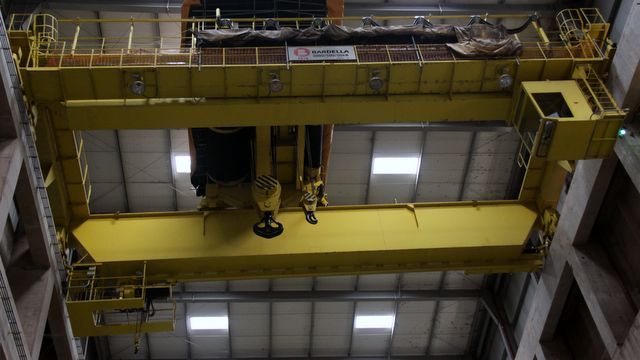
\includegraphics[width=\columnwidth]{figs/viagem/2015_04_28/UG/img_4989}
	\caption{Gantry crane and top hatch}
	\label{fig::portico}
\end{figure}

The environment may be briefly characterized by the blades dimensions,
element to coated; the ring chamber structure, which limits
the workspace of the robot; and the access.
%O ambiente pode ser resumidamente caracterizado pelas dimensões das pás,
%elemento a ser processado; características do aro câmara, estrutura que limita
% o espaço de trabalho do robô; e pelos acessos nos quais o sistema terá que
%utilizar.

\begin{itemize}
  \item \textbf{Turbine blades} - 420 stainless steel. Dimensions 2.5 x 2.5 m;
  \item \textbf{Ring chamber} - cylindrical structure 3.95 radius and metal
  surface;
  \item \textbf{Access}: 
  	\begin{itemize}
    	\item Top hatch - 35 cm diameter;
  		\item Bottom hatch - 80 cm diameter;
  		\item Suction tube - 20 x 20 m, access by river. 
  	\end{itemize}
\end{itemize}







\subsection{Robot tasks}\label{desc_taref}
This subsection describes the basic tasks of the robot for \textit{in situ}
turbine coating. Generally, the robot should be able to perform the coating task
as if the blade were not installed in the tubina, as it is done by Rijeza
company, in an autonomous way. As mentioned, the turbine blade should conform
to the template, hydraulic profile, before the coating process. Therefore,
another task is to perform the hydraulic profile mapping, build a 3D model and
analyze flaws.
%Esta subseção descreve as tarefas básicas do robô para o revestimento de
%turbinas \textit{in situ}. Em linhas gerais, o robô a ser desenvolvido deve ser
%capaz de realizar a tarefa de revestimento tal qual seria feita caso a pá não
% estivesse instalada na tubina e de uma maneira autônoma. A pá, antes de ser submetida ao
%processo de revestimento, deve estar em conformidade com o gabarito, perfil
% hidráulico de uma pá intacta. Portanto, uma tarefa do robô é realizar o mapeamento do perfil
%hidráulico, construir um modelo 3D e analisar imperfeições.


In case of deep blade deformations caused by cavitation and abrasion, the
repair by welding should be done manually or automatically. An operator can
manually perform the welding as there is no hard restrictions as the coating
process (accuracy, speed, load). However, the hostile and confined environment
can hinder the manual execution, thus welding can be also a robot task.
%Em caso de deformações, causados por cavitação e abrasão, estas precisam
%ser removidas manualmente ou de forma automatizada, possivelmente por
%soldagem. A tarefa de soldagem pode
%ser realizada por operador, manualmente, por não possuir todas as restrições
%da tarefa de revestimento (velocidade, precisão, carga e etc), porém o ambiente
%pode dificultar a operação de forma que a execução por um robô seja
%indispensável. 

If the blades conform to the hydraulic profile, the coating erosion
identification is made measuring the thickness of specific points on the
surface of the blade. An operator with a specific device can manually do this
process, efficiently in ten minutes. The coating erosion identification is not a
robot task.
%Após as pás estarem de acordo com o gabarito, faz-se a
%identificação do desgaste do revestimento, medindo sua espessura em pontos
%pontos específicos sobre a superfície da pá. Manualmente esse
%processo é realizado eficientemente em 10 min, justificando a não necessidade
% de esta ser uma tarefa do robô. 

The sandblasting process is normally required before the coating
operation, subsection~\ref{sandblasting}.Rijeza company performs the sandblasting manually, but there are studies and
companies performing sandblasting with robots. Thus sandblasting could be a
robot task.
%Em caso de necessidade de aplicação
%de novo revestimento, é necessária a remoção do revestimento antigo por
%jateamento, a fim de deixar a superfície rugosa e aumentar sua aderência. A
%tarefa de jateamento é atualmente realizada maualmente, mas também pode ser
%realizada pelo robô. Como ambos os lados da pá são revestidos, o jateamento
% deve ser realizado em ambos os lados. Vale ressaltar que, em teoria, pode-se aplicar revestimento por metalização sem retirar o último revestimento,
%porém esse processo ainda se encontra em fase de estudos na Rijeza.
%Segue-se o exemplo de empresas de aviação, onde existe a
%prática de retirar todo o revestimento antigo antes de aplicar o novo.

%Por fim, o robô deverá aplicar o revestimento como 
%forma de prevenir o dano causado pelos fenômenos abrasivos. O robô projetado
%para fazer o revestimento precisa preencher todos os requisitos discutidos na
%subseção~\ref{sec::desc_hvof} e ser adaptável ao ambiente, cujos as restrições
%são discutidos na subseção~\ref{sec::desc_contex}. 

Below, a summary of the task to be performed:
Tasks that can be performed manually:
%Das tarefas a serem relizadas, são destacadas as seguintes:
%Tarefas que podem ser executadas manualmente:
\begin{itemize}
  \item Blade damage inspection, for repair and for coating.%Inspeção e
  % análise de danos na pá, tanto para reparo quanto para revestimento.
  \item Repair.
  \item System mounting.%Montagem do sistema.
  \item Surface sandblasting.%Jateamento da superfície.
\end{itemize}

Tasks that can be performed by robot:%Tarefas que poderão ser executadas
% pelo robô:
\begin{itemize}
  \item Hydraulic profile modeling.%Modelar o perfil hidráulico.
  \item Calibration.
  \item Sandblasting.
  \item Repair.
  \item HVOF coating.
\end{itemize}




\section{State of the art}\label{sec:sota}
 
The study of the state of the art of robots for HVOF coating process on
hydraulic turbine blades covers systems that meet some of the following
requirements:
operation in hostile and confined environments; object manipulation with
at least 8.5 kg payload, 5 mm precision and $0.67 m/s$ speed; 2.5 m x 3.0 m
system workspace; and the ability to operate on complex 3D geometry surfaces.
The robots were divided by fixation technologies.
%O estudo do estado da arte de robôs para a realização de HVOF em pás de
% turbinas hidráulicas contempla os sistemas que atendem a alguns dos requisitos: operar
%em ambientes de alta periculosidade; capacidade de carga para os dispositivos
% HVOF; manipular a pistola HVOF com velocidade de $0.67 m/s$; precisão de 5mm; ter
%área de trabalho de 2.5 m x 2.5 m; e operar sob superfícies 3D de geometria
%complexa. As soluções foram divididas em subseções de acordo com as tecnologias
%de fixação dos robôs.


 
\subsection{Robots on rails}\label{sec::rail}
In industry, HVOF coating processes are performed by robotic manipulators,
which offer tasks versatility and large workspace, required for this
type of application. Meanwhile, a robotic arm capable of coating all the turbine
blade surface on a fixed position is not compact or mobile, and hard to be
mounted/unmounted. A prismatic joint coupled to a rail is a common strategy for
extending the robot working space, without adding weight to the manipulator,
and the rail can use the structures in the environment as a support.
%Na indústria, a automatização de processos de metalização, é
%normalmente realizada com a utilização de manipuladores robóticos, pois oferece
%a versatilidade de tarefas e espaço de trabalho necessários para esse
%tipo de aplicação. Entretanto, um sistema composto por um braço robótico capaz
%de operar em toda a extensão da superfície da pá da turbina hidrelétrica
%não é compacto, nem móvel o suficiente para ser instalado e desinstalado para a
%operação de manuntenção \textit{in-situ}.


%A introdução de uma junta prismática acoplada a um trilho é uma estratégia para
%reduzir o tamanho e o peso de um manipulador robótico.  Assim, é possível
% estender o espaço de trabalho do robô, sem adicionar peso ao manipulador, uma vez que o
% trilho pode usar as estruturas presentes no ambiente como apoio. 


%Na literatura foram encontradas duas soluções para aplicações de manutenção e
%inspeção, como solda, específicas para o contexto de turbinas hidráulicas. As
%aplicações diferem, principalmente, na estratégia de fixação do sistema
%de trilhos.
%O Roboturb \citep{roboturb} realiza a fixação
%diretamente na pá do rotor, enquanto o robô Scompi \citep{scompi} utiliza um
% trilho fixado em
%estruturas adjacentes à pá ou peça a ser reparada.

The Roboturb \citep{roboturb} is a robotic manipulator composed of six
revolution joints and one prismatic joint coupled to a flexible rail.
%figure~\ref{fig::roboturb}. 
The robot performs welding, filling cavities generated by erosion. The rail
may be shaped and then fixed to the blade surface by a passive system of
suction cups. The robot has two end-effectors: an optical sensor for erosion
inspection; and a welding tool, a PWH-4A plasma torch with automatic feeder.
%O Roborturb \citep{roboturb} consiste em um manipulador robótico com seis
% juntas de revolução e uma junta primsática acoplada a um trilho flexível, como pode ser observado
%na figura \ref{fig::roboturb}, utilizado para o preenchimento de cavidades
%geradas por cavitação.
%O trilho pode ser conformado e, então, fixado à superfície da pá por meio de um
%sistema passivo de ventosas ou ímãs. O robô tem a possibilidade de utilizar
% dois efetuadores distintos, o primeiro consiste em um sensor ótico para inspeção do 
%estado de erosão da pá e o segundo consiste em uma ferramenta de solda do 
%tipo tocha plasma PWH-4A com alimentador automático de arame, responsável pelo 
%depósito de solda para o preenchimento das cavidades identificadas pelo
% sistema.


%TODO Abelha: Posicionar corretamente as figuras
%    \begin{figure}[h!]	
%		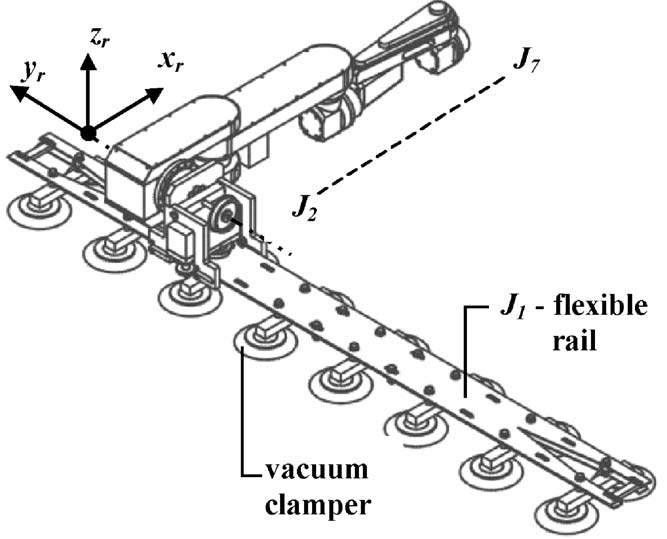
\includegraphics[width=\columnwidth]{figs/trilhos/roboturbpaper}
%		\caption{Roboturb - Robotic manipulator on rail}
%		\label{fig::roboturb}
%	\end{figure}
%	\begin{figure}[h!]
%		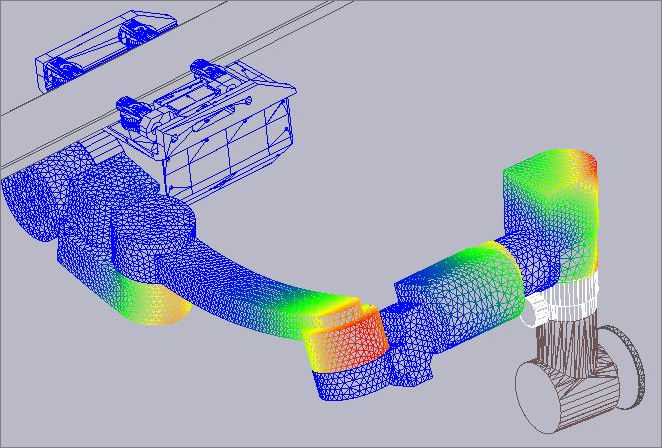
\includegraphics[width=\columnwidth]{figs/trilhos/scompi}
%		\caption{SCOMPI - Manipulador robótico sobre trilhos rígidos}
%		\label{fig::scompi}
%	\end{figure}

The Scompi robot \citep{scompi}%, figure~\ref{fig::scompi}, 
is a multipurpose manipulator, designed to perform repairs on \textit{Francis}
type turbines, as welding and grinding. It has six degrees of freedom: a robotic
manipulator with five revolution joints; and a prismatic joint, coupled to
curved rails that are designed specifically for each application.
%Por sua vez, o robô Scompi \citep{scompi}, fig \ref{fig::scompi}, é um
%manipulador multipropósito projetado para realizar reparos em turbinas do tipo
% \textit{Francis}, como solda e esmerilhamento das pás. O sistema possui seis graus de liberdade,
%sendo consitituído por um braço robótico com cinco juntas de revolução, e o
%último grau de liberdade proveniente de uma junta prismática que percorre um
% sistema de trilhos retos ou curvos que são projetados para cada aplicação especificamente. 


%Sistemas baseados em trilhos tem como maior benefício a redução do tamanho e,
%consequentemente, do peso do manipulador necessário para a execução de tarefas
%em um espaço de trabalho que englobe toda a superfície da pá.
%Essa redução proporciona facilidade de transporte do robô até o interior da
%turbina e também possibilita o projeto de manipuladores que tenham a rigidez
%necessária para a realização das tarefas desejadas. 

Fixed robotic manipulators which meets the HVOF payload and
workspace requirements would be too heavy. Systems based on rails fixed
on the blade itself, require rail handling as the entire
blade surface should be coated and the area in which the rail is fixed is not in
the robot workspace. In addition, rail systems fixed on adjacent structures
should considerate the installation conditions and balance the cost-benefit
of installation/removal rail, and robustness.
%Manipuladores robótico fixos, rígidos o suficiente para aguentar as forças
% intrínsecas ao processo de metalização e com espaço de trabalho necessário para trabalhar em
%toda a extensão da superfćie da pá seriam muito pesados.
%Entretanto, sistemas baseados em trilhos com fixação na própria pá do rotor,
% necessitam que o trilho seja movido caso se deseje que toda a superfície da pá sofra
%manuntenção, uma vez que a área em que o trilho está apoiado não pertence ao
% espaço de trabalho do robô. Em adição, sistemas com fixação de trilhos nas estruturas
%adjacentes à pá devem atentar as condições para a instalação disposta pelo
%ambiente para equilibrar a relação de custo benefício entre facilidade de
%instalação/remoção do trilho e a robustez.
The system advantages are: 1) manipulator size reduction; 2) manipulator
weight reduction. The disadvantages are: 1) rail mounting and unmouting; 2) rail
handling if fixed on the blade. 
\subsection{Climbing robots}\label{sota_climbers}
Climbing robots are systems capable of supporting its own weight against
gravity, moving in simple or complex geometric structures, such as
walls, ceilings and roofs, turbine blades and nuclear plants.
Generally, clim\-bers are used to provide operational efficiency in harsh
environments, and to increase safety. Some applications for
climbing robots are:
skyscrapers inspection and cleaning, storage tanks diagnosis in nuclear
power plants, ship's hull and turbine welding and
maintenance \citep{armada2003application}.
%Robôs escaladores são sistemas capazes de sustentar seu próprio peso contra a
%gravidade, movendo-se em simples ou complexas estruturas geométricas, como
%paredes, tetos e telhados, palhetas de turbinas e plantas nucleares.
%Essa classe de robôs oferece eficiência operacional em ambientes
%de alta periculosidade, sendo utilizados visando saúde e segurança dos
%trabalhadores, como em inspeção e limpeza de arranha-céus, diagnóstico de
%tanques de armazenamento em plantas nucleares, solda e manutenção de cascos de
%navios e palhetas de turbinas \citep{armada2003application}. 

The major challenges in climbers development are mobility, adhesion,
power consumption, load capacity, and weight. In \cite{modular} and \cite{climbsurv},
climbers are divided into types of locomotive mechanisms: legs; walker; translation; wheels; tracks;
advance by arms; cable-driven; and biomimetics. And adhesion types:
suction or pneumatic; magnetic; electrostatic; chemical; gripping; and hybrid.
%Os grandes desafios nos projetos de sistemas escaladores são mobilidade e
%aderência, além de consumo de energia, capacidade de carga e peso. Em
%\cite{modular} e \cite{climbsurv}, os robôs escaladores são divididos em tipos
%de locomoção:
%pernas; como andador; utilizando segmentos deslizantes; rodas; esteiras; avanço
%pendurado por braços; por cabos; e biomimética. E categorias de adesão: sucção
%ou pneumática; magnética; eletrostática; química; preensão; e híbrida.

The following climber robots were investigated:
%No caso específico deste estudo da arte, destacam-se os robôs escaladores com
% as seguintes aplicações:

\begin{itemize}
  \item \textbf{Ships and turbines}: RRX3 for welding
   \citep{rrx3}, \textit{Climbing Robot for Grit Blasting} for cleaning
   \citep{crgb}, ICM Robot for inspection \citep{icm}, and RIWEA \citep{riwea};
  \item \textbf{Industrial}: ROME II \citep{roma} and CROMSCI \citep{CROMSCI}, both for inspection;
 % \item \emph{petrochemical plant}: TRIPILLAR \citep{tripillar} for inspection.
\end{itemize}

The RRX3 (Fig.~\ref{rrx3}), Daewoo Shipbuilding \& Marine Engineering, is a
robot for ship's hull welding with manipulator. It has a gripping adhesion
type, a translation locomotion type (sliding segments), and
longitudinal locomotion by wheels. The RRX3 robot has a 1.5 m manipulator with
three prismatic joints and three revolution joints  (3P3R) for welding operation. The system weighs 120 kg with 5
kg payload, it has a manipulator with welding tool.
%O RRX3 (figura~\ref{rrx3}), Daewoo Shipbuilding and Marine Engineering, é um
%robô para a soldagem de casco de navios. Possui adesão por preensão, locomoção
% transversal utilizando segmentos deslizantes e locomoção longitudinal por rodas. Possui um manipulador de 1.5 m com três juntas
%prismáticas e três juntas de revolução (3P3R) para a operação de soldagem. 

%RRX 3 main characteristics are: base and manipulator with
%120 kg and 5 kg of payload, respectively; accurately
%millimeter manipulator and low speed end effector; robustness; welding tool
%operation; limited translation type locomotion.
%As características principais do robô são: base e manipulador com
%capacidades de carga de 120 kg e 5 kg, respectivamente; manipulador com
% precisão milimétrica e efetuador de baixa velocidade; robustez para operar em ambiente de
%alta periculosidade; opera instrumento de solda; e locomoção transversal é
%restrita à aplicação.

\begin{figure}[ht]
\centering
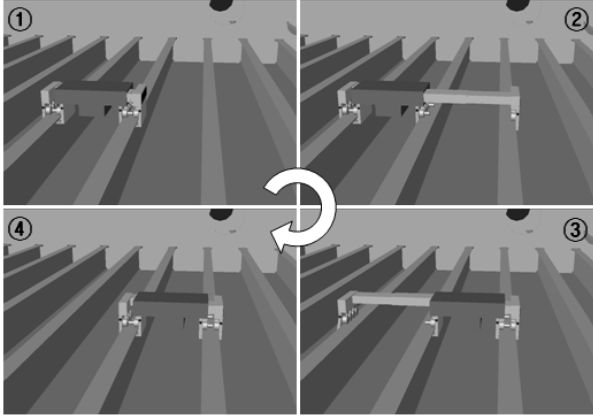
\includegraphics[scale=0.25]{figs/climbers/RRX3_moving.jpg}
\caption{RRX3 translation locomotion.}
\label{rrx3}
\end{figure}

The \textit{Climbing Robot for Grit Blasting} (Fig.~\ref{grit}), %, 
University of Coruna, is a robot for abrasive blasting application in ships. The
robot moves by two sliding platforms with magnetic adhesion. The platforms have relative motion
between them and can rotate to compensate ship's hull curvatures or to
deflect objects. The abrasive system is similar to HVOF, but the robot
locomotion is not applicable to complex structures.
%O \emph{Climbing robot for Grit Blasting} (figura~\ref{grit}), University of
%Coruna, é um robô para jateamento abrasivo em navios. O robô utiliza duas
% plataformas deslizantes com sistema de adesão por ímã magnético. Os módulos apresentam movimentação relativa entre si e pode rotar
%para compensar as curvaturas do casco do navio ou desviar de objetos. 

%The \emph{Climbing robot for Grit Blasting} main characteristics are:
%abrasive system similar with HVOF; accurately
%millimeter movement; locomotion not applicable to complex structures; no
%manipulator.
%As características principais do robô são: base com
%capacidade de carga de sistema abrasivo semelhante a HVOF; base com
%locomoção de precisão milimétrica; locomoção ampla, mas não aplicável a
%estruturas complexas; e não possui manipulador, sendo necessário percorrer todo
%o casco.

\begin{figure}[ht]
	\centering
	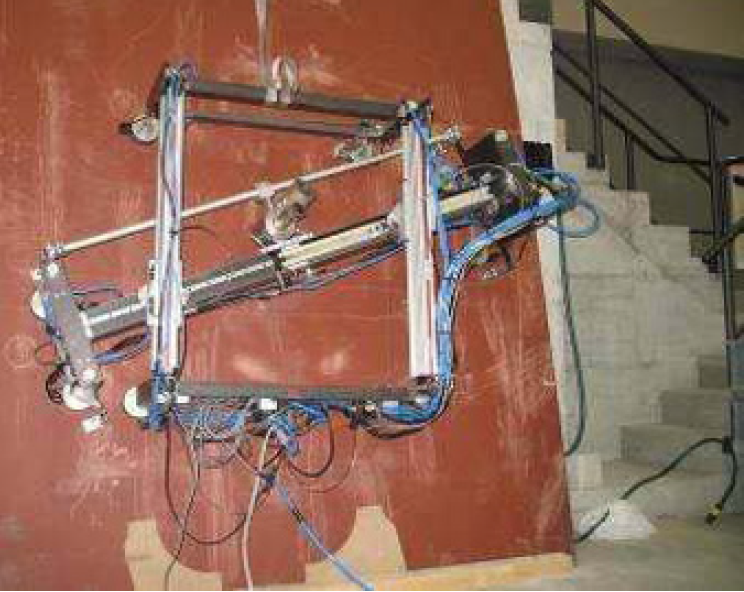
\includegraphics[scale=0.3]{figs/climbers/grit.png}
	\caption{Climbing robot for Grit Blasting}
	\label{grit}
\end{figure}


\textit{The Climber} (Fig.~\ref{icm})
, ICM Robotics, is an inspection robot for
wind turbines, coating removal, surface cleaning and coating application.
It has pneumatic adhesion and locomotion by tracks. It has 25 kg base payload,
and a small-sized low speed manipulator. The locomotion type presents
restrictions to some curvatures.
%\emph{The Climber} (figura~\ref{icm}), ICM Robotics, é um robô para inspeção de
%turbinas eólicas, remoção de revestimento, limpeza de superfície, e aplicação
% de revestimento.
%Possui adesão pneumática (sucção) e locomoção por esteiras. 

%\emph{The Climber} main characteristics are: 25 kg base payload; accurately
%millimeter movement; a modular manipulator can be attached to the base; small
%size manipulator and low speed; locomotion type presents restriction to
%some curvatures.
%As características principais do robô são: base com capacidade de carga de 25
%kg; base com locomoção de precisão milimétrica; manipulador modular pode ser
%acoplado à base; manipulador de dimensão reduzida e baixa velocidade; e
%locomoção apresenta restrição a algumas curvaturas acentuadas.

\begin{figure}[ht]
	\centering
	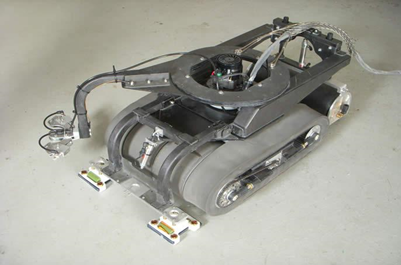
\includegraphics[scale=0.8]{figs/climbers/icm.png}
	\caption{\textit{The Climber}}
	\label{icm}
\end{figure}

The Rome II%(figura~\ref{roma2})
, University Charles II of Madrid, is an inspection robot for complex
environments. It has pneumatic adhesion and moves like a caterpillar
(biomimicry). Rotation and planning trajectory are performed optimally to
ensure stability and obstacle avoidance.
%O ROMA II (figura~\ref{roma2}), Universidade Carlos II de Madrid, é um robô
% para inspeção de ambientes complexos. A sua tecnologia de adesão é pneumática (sucção) e
%locomove-se como uma lagarta (biomimética). Sua movimentação e planejamento de
%trajetória são realizados de maneira ótima de forma a garantir estabilidade e
%evitar obstáculos. 

%The Rome II main characteristics are: high payload capacity; accurately
%millimeter movement; no manipulator; locomotion for complex environments.
%As características principais do robô são: base com grande capacidade de carga;
%base com locomoção de precisão milimétrica; não possui manipulador; locomoção
% em ambientes de grande complexidade.

%\begin{figure}[ht]
%\centering
%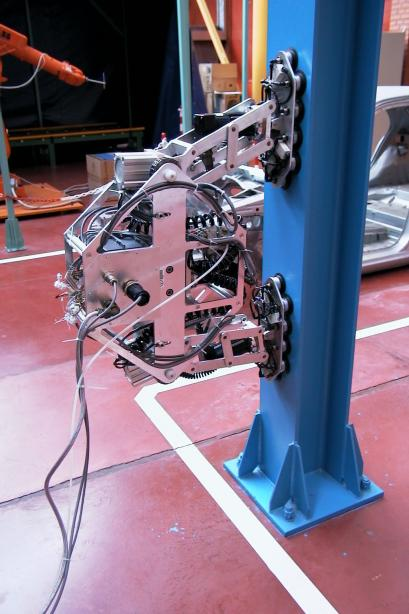
\includegraphics[width=8.4cm]{figs/climbers/roma2.jpg}
%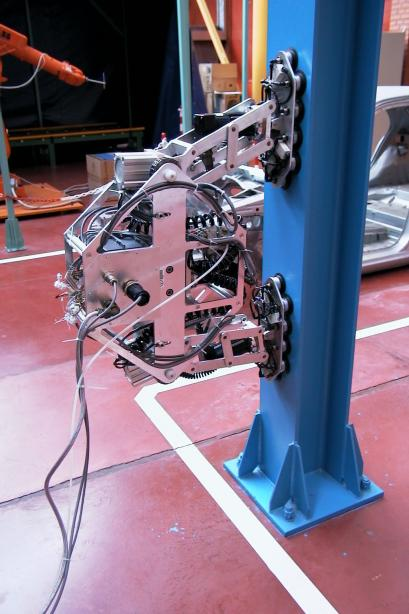
\includegraphics[width=4.2cm,height=4.2cm]{figs/climbers/roma2.jpg}
%\caption{ROMA II.}
%\label{roma2}
%\end{figure}
CROMSCI% (figure~\ref{cromsci})
, Kaiserslautern University of Technology, is an
inspection and autonomous robot for large concrete walls, as
pillars of bridges and dams. Its adhesion system is composed of seven vacuum
chambers (suction), valves and pressure sensors for system control. The
locomotion system has omnidirectional wheels.
%CROMSCI (figura~\ref{cromsci}), Kaiserslautern University of Technology, é um
%robô autônomo para inspeção de grandes paredes de concreto, como pilares de
% pontes, barragens. Seu sistema de adesão é composto por sete câmaras de vácuo (sucção), com um sistema
%de controle por válvulas e sensores de pressão para reagir rapidamaente a
%condições adversas. Locomove-se com rodas omnidirecionais para locomoção.

%The CROMSCI main characteristics are: low payload capacity; accurately
%millimeter movement; no manipulator; low speed.
%As características principais do robô são:
%base com pouca capacidade de carga; base com locomoção de precisão milimétrica;
% não possui manipulador; e apresenta baixa velocidade.

%\begin{figure}[ht]
%\centering
%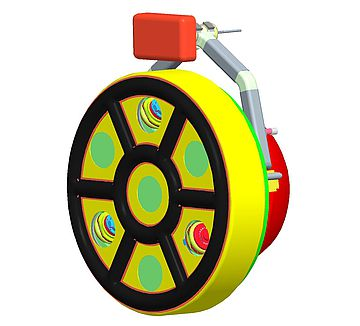
\includegraphics[width=8.4cm]{figs/climbers/cromsci.jpg}
%\caption{The CROMSCI robot.}
%\label{cromsci}
%\end{figure}

% TRIPILLAR, Ecole Polytechnique Federale de Lausanne, is a small inpection robot
% (96 x 46 x 64 mm) for petrochemical plants. Its adhesion is done by magnetic
% legs on a caterpillar triangular shape, and it moves by tracks.

% A specific case of climbers is the \textit{cabling robots}, which use a set
% of cables to ensure its proper positioning in its working area. The cables provide
% manipulator range improvement, decrease the adhesion complexity and reduce the
% weight carried by the robot. As an example, the \textit{torboMate} is a climber
% with magnetic adhesion, it can have two or more emitting jets with 4000 bar of
% supply capacity. It has 45 kg and reaches 20 m/min speed \citep{torbo}.

RIWEA is a purely cabling robot, as it has no other type of position
adjustment, for cleaning wind power turbines. It is an open frame concept robot
which uses four ropes to move up and down. It has five main parts, which
automatically adjust to the blade surface during its movement
\citep{jeon2012maintenance}. Its greatest advantage lies in the ability to adapt
to the curvature of the blade while maintaining a foothold on it, and it is also
less susceptible to vibration.

Climbing robots are widely applicable, have different adhesion solutions and
mobility. There is not, so far, a climber that fulfills all the HVOF
requirements for the large hydropower turbine's blades, but some of the
systems, such as \textit{The Climber} (ICM Robotic), can generate complete
solutions with adaptations.
%Os robôs escaladores são utilizados em diversas aplicações e possuem diferentes
%soluções de aderência e locomoção, como foi exposto nesta subseção. Não há,
%até o momento, um robô escalador que possui todas as características
%exigidas para a tarefa de HVOF em pás de turbinas, porém a adaptação de
%alguns desses sistemas, como \emph{The Climber} da ICM Robotic, pode gerar
%soluções completas.

The advantages of climbers are: easily installation, small-sized
manipulator, small base, lightweight, autonomy; and the disadvantages are:
complex locomotion system, complex mechanics, manual installation on blade,
required a well-developed safety system, it generally has limited battery or
an umbilical management system. 
%As vantagens e desvantagens para solução de robôs escaladores são:
%\textbf{Advantages:}
%\begin{itemize}
%  \item Easily installation;
%  \item Small size manipulator, since robot moves on blade;
%  \item Small base;
%  \item Small weight;
%  \item Autonomy while operating; 
%\end{itemize}
%and disadvantages 
%\textbf{Disadvantages:}
%\begin{itemize}
%  \item Complex locomotion system with obstacle avoidance and path
%  planning;
%  \item Complex mechanics, as robot should be able to support its weight plus
%  the manipulator and the HVOF spary gun;
%  \item Robot must be manually installed on each blade or a complex locomotion
%  system by arms should be developed;;
%  \item Robot safety system must be well developed;
%  \item Limited battery or umbilical management system for mobile robots;
%\end{itemize} 
%\subsection{Robôs cabeados}
São classificados como robôs cabeados quaisquer sistemas robôticos que façam
uso de um conjunto de cabos e/ou cordas para auxiliar ou mesmo garantir seu
posicionamento adequado na sua região de trabalho. Sendo assim, robôs cabeados
podem possuir outros métodos de fixação em conjunto com seu cabeamento.

A idéia do uso de um sistema de cabos surge naturalmente quando o deslocamento
se mostra majoriamente restrito a um plano vertical e não há exigência de
grandes velocidades de deslocamento. O sistema é usado como forma de reduzir o
preso e melhorar o desempenho de um braço mecânico de mesmo alcance, ou diminuir a complexidade e
a força de aderência necessária para um escalador.

Para exemplificar essa categoria foram selecionados dois robôs. O
\textit{torboMate} é um escalador que possui adesão magnética que o
permite caminhar livremente. Pode ter dois ou um
emissor de jatos com capacidade para abastecimento em até 4000 bar. Possui 45 kg
e atinge uma velocidade de até 20 m/min \citep{torbo}.

\begin{figure}[ht]
	\centering
	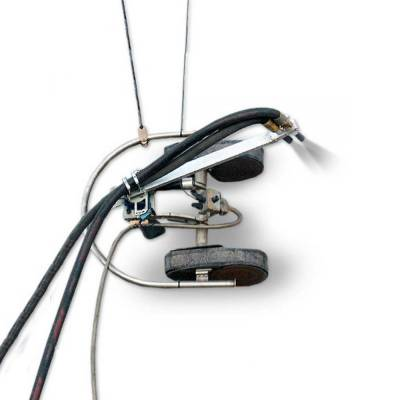
\includegraphics[width=8.4cm]{figs/cables/torbo}
	\caption{Robô TorboMate "Crawler", \cite{torbo}}
	\label{fig:cables:torbo}
\end{figure}

RIWEA é um robô puramente cabeado, no sentido em que ele não possui nenhum
outro tipo de forma de ajuste de posição além do sistema de cabos. É um
conceito de robô de estrutura aberta que faz uso de quatro cordas para se
deslocar verticamente \citep{jeon2012maintenance}. Seu maior diferencial reside
na capacidade de se adaptar a curvatura da pá mantendo sempre um ponto de apoio
sobre ela, sendo também menos suceptivel a vibrações \citep{riwea}.

\begin{figure}[!h]
	\centering
	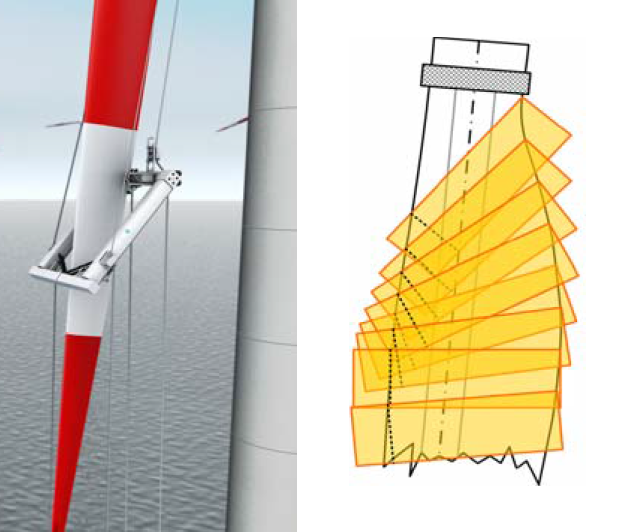
\includegraphics[width=8.4cm]{figs/cables/riwea}
	\caption{Robô RIWEA, sua cinemática adaptável ao formato da pá, \cite{riwea}}
	\label{fig:cables:riwea}
\end{figure}

Em geral, podemos sumarizar as caraterísticas do robôs cabeados segundo as
seguintes vantagens e desvantagens.

\textbf{Vantagens:}
\begin{itemize}
  \item Redução da carga sobre a fixação do robô / maior capacidade de carga.
  \item Alcance do robô pelo cabeamento pode ser estendido a baixo custo.  
\end{itemize}

\textbf{Desvantagens:}
\begin{itemize}
  \item Complexidade do sistema de gestão do cabeamento.
  \item Necessidade de um ponto de apóio superior para fixação dos cabos.
\end{itemize}



%\subsection{Manipulador com base esférica}
A research and development project was presented in
\cite{motta2010prototype} to propose methodology, simulation and
the steps for constructing a robotic system to recover damage
in hydraulic turbines blades. The robotic system does
repair using the arc welding technology before held
manually in highly dangerous environments with temperatures ranging
between $ 40^o C$ and $ 99^o C$, in a 10 hours operation.
%Um projeto de pesquisa e desenvolvimento foi apresentado em
%\cite{motta2010prototype} com o objetivo de propor metodologia, simulação e
%os passos para construção de um sistema robótico para recuperar danos materiais
%em pás de turbinas hidráulicas. O sistema robótico faz
%reparo utilizando a tecnologia de soldagem a arco elétrico, antes realizada
%manualmente em ambientes de alta periculosidade com temperaturas que variam
%entre $40^o C$ e $99^o C$, e operações que duram em torno de 10 horas. 

The robot must meet the following requirements:
\begin{itemize}
   \item ability to operate in any position: horizontal, vertical,
   reversed;
   \item light weight for portability and blade fixation;
   \item stiffness to deflection: payload on the wrist occurs in any
   direction and extension;
   \item high precision;
   \item parts availability on the market;
   \item user interface;
   \item large workspace;
   \item adhseion to the hydraulic turbine blades.
\end{itemize}

%O robô deve atender aos seguintes requisitos:
%\begin{itemize}
%  \item Capacidade de operar em qualquer posição: horizontal, vertical,
%  invertida;
%  \item Pouco peso para portabilidade e fixação às pás;
%  \item Rigidez à deflexão: carga no punho do manipulador ocorre em qualquer
%  direção e extensão;
%  \item Grande precisão;
%  \item Disponibilidade de peças no mercado;
%  \item Controle com interface de usuário;
%  \item Grande área de trabalho;
%  \item Facilidade de adesão às pás de turbinas hidráulicas.
%\end{itemize}

The solution to the robotic system has spherical topology as can be
shown in figure~\ref{fig: spherical} and the following characteristics:
%A solução para o sistema robótico apresenta topologia esférica, como pode ser
%visto na figura~\ref{fig:esferico} e características:

\begin{figure}[ht]
\centering
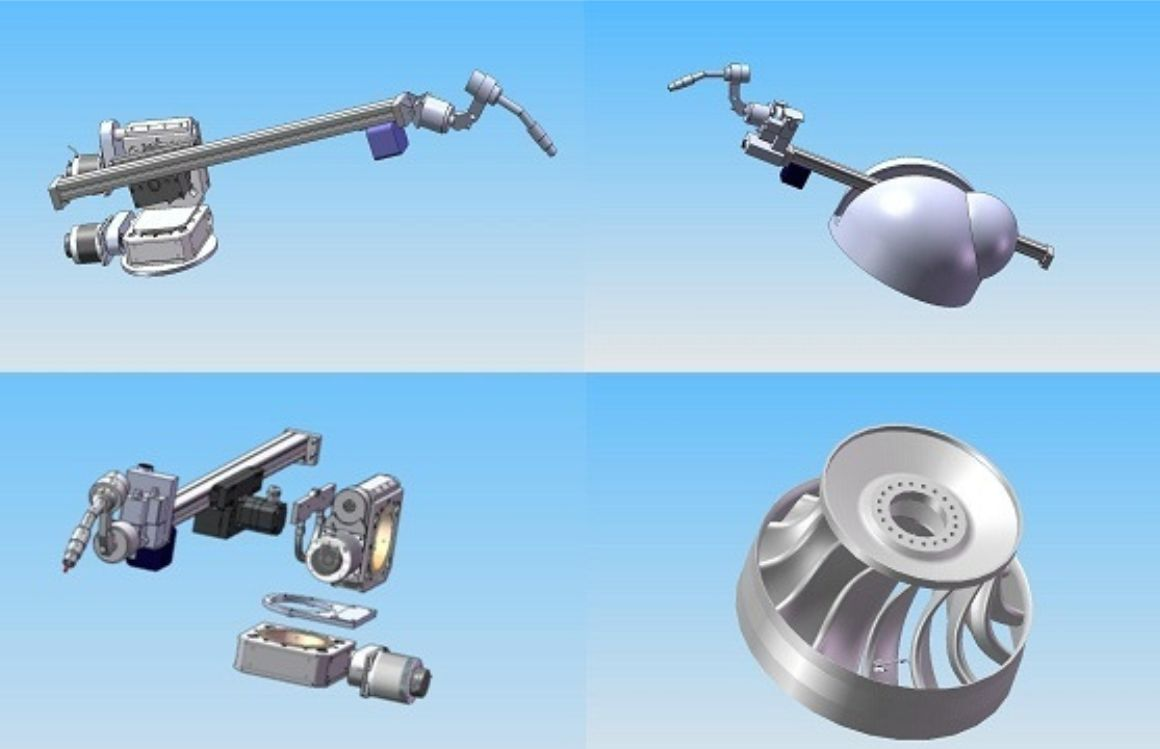
\includegraphics[width=8.4cm]{figs/esferico/esferico.jpg}
\caption{Illustration of the robotic system with spherical base}
\label{fig:esferico}
\end{figure}

\begin{itemize}
   \item manipulator with three DOF (2R1P) and wrist with two DOF (2R);
   \item 3D surface mapping with laser scanner;
   \item embedded electronics;
   \item arc welding;
   \item blade adhesion by magnetic or suction devices;
   \item low cost;
   \item ring-shaped workspace with 2.5 m, and 60 cm height;
   \item 30 kg weight and dimensions 30 x 25 x 100 cm;
   \item autonomous manipulator;
\end{itemize}

%\begin{itemize}
%  \item Três (3) graus de liberdade no manipulador (2R1P) e dois graus de
%  liberdade no punho (2R);
%  \item Mapeamento de superfície 3D com laser;
%  \item Eletrônica embarcada;
%  \item Soldagem por arco elétrico;
%  \item Fixação nas pás por dispositivos magnéticos ou de sucção;
%  \item Baixo custo;
%  \item Área de trabalho em forma de anel com 2.5 m e 60 cm de altura;
%  \item Peso 30 kg e dimensões 30 x 25 x 100 cm;
%  \item Robô com manipulador autônomo;
%\end{itemize}

The robotic manipulator system with spherical base is a compatible solution
for the HVOF application in hydraulic turbine blades, since its
original application is blade repair by arc welding, same environment and
similar challenge. All the system advantages and features are applicable to
the solution of a HVOF system. However, there are particular challenges in the
HVOF process, which are disadvantages of the solution:

%O sistema robótico de manipulador com base esférica apresenta solução
% compatível para a aplicação de HVOF em pás de turbinas hidráulicas, já que sua aplicação
%original é soldagem das pás, semelhante ao desafio deste artigo. Todas as suas
%características são vantagens e aplicam-se à solução de um sistema para HVOF.
%Há, porém, desafios particulares na metalização das pás e que são desvantagens
%da solução:


\textbf{Disadvantages:}
\begin{itemize}
   \item The HVOF must be performed in the entire blade. Therefore, the
   positions of the system must be manually changed at least 2 times per blade
   side, and must be moved blade to blade;
   \item The end effector must process the blade with great speed, as
   required by the HVOF.
\end{itemize}

%\textbf{Desvantagens:}
%\begin{itemize}
%  \item A metalização deve ser realizada em toda a pá. Portanto, o sistema
%  deverá ser manualmente trocado de posição, pelo menos 4 vezes (duas posições
%  para a frente e duas posições para a região de trás). E deve ser trocado de
  % pá em pá;
%  \item O efetuador deve percorrer a pá com grande velocidade, como exige o
%  processo de metalização.
%\end{itemize}

\section{Design of a robotic system for \textit{in situ} HVOF}\label{sec:projeto}

The autonomous system design for HVOF in hydraulic turbine blades include
solutions that meet all the application's requirements. Thus, the envisioned
robots of this section merge some technologies exhibited in
section~\ref{sec:sota} in the context of the Jirau hydroelectric dam.

%O projeto de robôs autônomos para HVOF em pás de turbinas hidráulicas contempla
%as soluções que atendem a \textbf{todos} os requisitos da aplicação. Dessa
%forma, serão idealizados robôs com a fusão das tecnologias expostas na
%seção~\ref{sota} e no contexto da usina hidrelétrica de Jirau. 

In section~\ref{sec::consideracoes}, the Runner area accesses were described
and their restrictions are essential for the elaboration of the solution.
This section is divided into robotic solutions for both accesses, since they
are the most important development restriction, as they limit robot's
dimensions, features, and demand different logistics.

%Na seção~\ref{sec::consideracoes}, os acessos ao aro câmara foram
%descritos e suas restrições são fundamentais para a elaboração da solução.
%Esta seção é dividida em soluções de sistemas robóticos para os dois tipos
%de acessos, já que estes são o fator que mais restringe o desenvolvimento do
%sistema robótico por limitar suas dimensões, funcionalidades, e exigir a
%idealização conjunta de uma logística de acesso e movimentação do robô pelo aro
%câmara.
 
\subsection{Top hatch}
The top hatch, localized at the top of the arc chamber, has only 350 mm
diameter, which is a challenge when thinking about using it as a robotic system access
point. Furthermore its proximity to the blades and the free space outside the
arc chamber create interesting possibilities for its use. Using the top hatch as
the access for robot has the follwing advantages: robot fixation stability,
reference point (facilitating localization system, mapping, control and
calibration), built logistics (conveyor gantry to position the robot and the
HVOF system); and the following disadvantages: difficulty in finding robots of
such size (350 mm diameter), the robot must be removed to rotate the blades, and
it is not a general solution (specific to Jirau installations).
%Essa escotilha localizada no topo do aro câmara possui uma abertura de apenas
%35 cm de diâmetro, o que cria um desafio quando se pensa em utiliza-la como
%ponto de acesso para um robô. Por outro lado sua proximidade às pás e a área
% livre fora do aro câmara criam possibilidades interessantes para seu uso.

%\textbf{Advantages}
%\begin{itemize}
%  \item robot fixation stability
%  \item reference point, facilitating localization system, mapping, control and
%  calibration
%  \item built logistics: conveyor gantry to position the robot and the
%  HVOF system
%\end{itemize}

%\textbf{Disadvantages}
%\begin{itemize}
%  \item difficulty in finding robots of such size (35 cm diameter)
%  \item during the operation, the robot must be
%  removed to rotate the blades
%  \item not a general solution, specific to Jirau
%\end{itemize}

The simplest solution to this access is to use an industrial manipulator.
The choice of the robot is primarily associated with reach, but only a small
share of commercial robots has the dimension to fit the top hatch. Thus, the
study was focused on the KUKA Light Weight (LBR iiwa 14 R820), robot whose base
diagonal is less than 350 mm.

%A solução mais simples para este acessso é a utilização de um robô industrial
%comercial. A escolha do robô está primariamente associada ao seu alcance. Por
% outro lado, apenas uma pequena parcela dos robôs comerciais possuem a dimensão necessária para
%atravessar a escotilha. Sendo assim, o estudo foi direcionada para o uso do
%KUKA Light Weight (LBR iiwa 14 R820), robô cuja diagonal da base é inferior aos
%35 cm da escotilha.


The LBR R820 weighs 30 kg, has seven joints and has 14 kg payload, enough to
carry the coating equipment. However, further studies are needed to validate
the robot, as the speed and precision requirements when coating.

%O LBR R820 pesa 30 kg, possui 7 eixos e suporta carga de 14kg,
%suficiente por uma pequena margem para carregar o equipamento de
%revestimento. Entretanto, são necessários estudos aprofundados para valida-lo,
%como os requisitos de velocidade e precisão quando percorrendo a trajetória
%para a realização do revestimento.

To place the LBR R820 in a position where it is able to process all the
blade, a hinged base model was proposed. The base consists of three telescopic
links interconnected by a revolute joint, and the first link is attached to the
top hatch itself. To cover the entire blade, the base must be able to assume different angles with
respect to the insertion axis, the links must be telescopic type with
prismatic joints.  

The base's structure would consist of cylinders with maximized diameter and
small thickness, which features a high polar moment of inertia and light weight,
providing great bending stiffness, and minimizing positioning errors and
excessive vibration. A recirculating ball actuators were chosen for low
backlash and high precision. Figure~\ref{fig::baselbr} shows the manipulator'
base concept in two configurations: retracted and extended.

%A base consiste em 3 braços
%telescópicos que permitem a extensão do sistema para prover o alcance
%necessário ao manipulador e o recolhimento para uma configuração incial que
%permita a entrada do manipulador no aro câmara com segurança, sem o risco de
%choques ou interferências indesejadas. Além disso, uma junta rotativa oferece
% mais um grau de liberdade para o sistema, facilitando o acesso do manipulador à toda ar
%superfície da pá. 

%Os atuadores da base são acionados eletricamente e possuem sensores de
%posicionamento. Atuadores de esferas recirculantes foram escolhidos devido à
%baixa folga e precisão elevada. A estrutura da base é composta por cilindros de
%diâmetro maximizado e pequena espessura, o que oferece um momento de inércia
%polar elevado e baixo peso, fornecendo grande rigidez à flexão e minimizando
%erros de posicionamento e vibração excessiva. A
% figura~\ref{fig::base_recolhida} e a figura~\ref{fig::base_extendida} apresentam o conceito da base do manipulador em duas configurações: recolhida (configuração
%de entrada) e estendida (configuração de operação).

\begin{figure}[h!]
\centering
	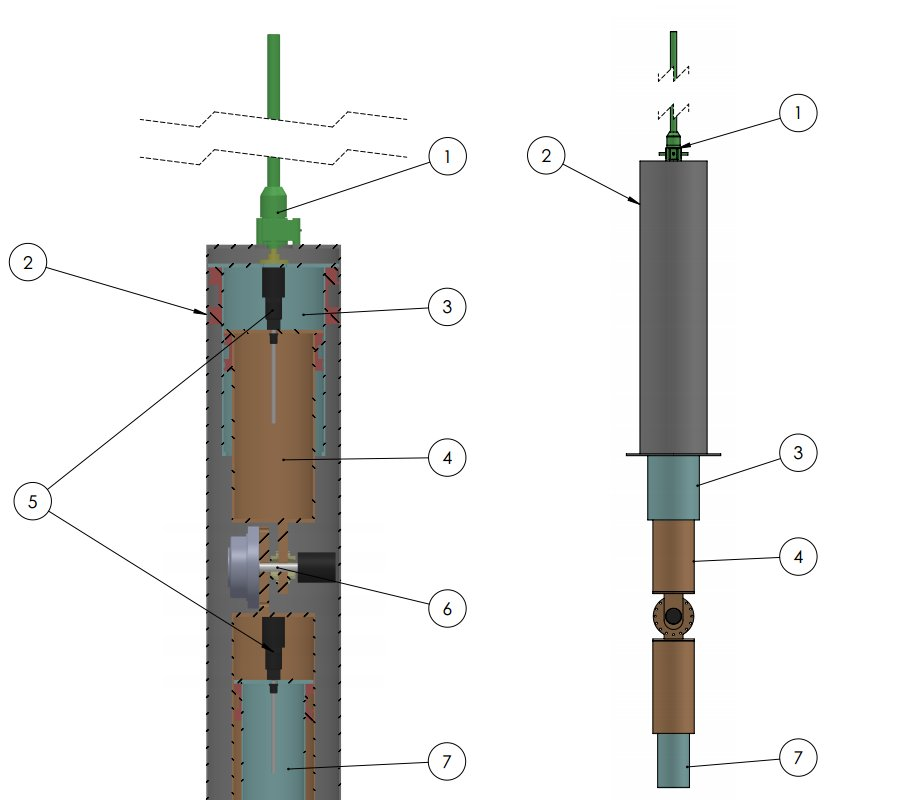
\includegraphics[width=\columnwidth]{figs/estudo/solid/baselbr.jpg} 
	\caption{Initial and extended configuration of the base.}
	\label{fig::baselbr}
\end{figure}

%\begin{figure}[h!]
%\centering
%	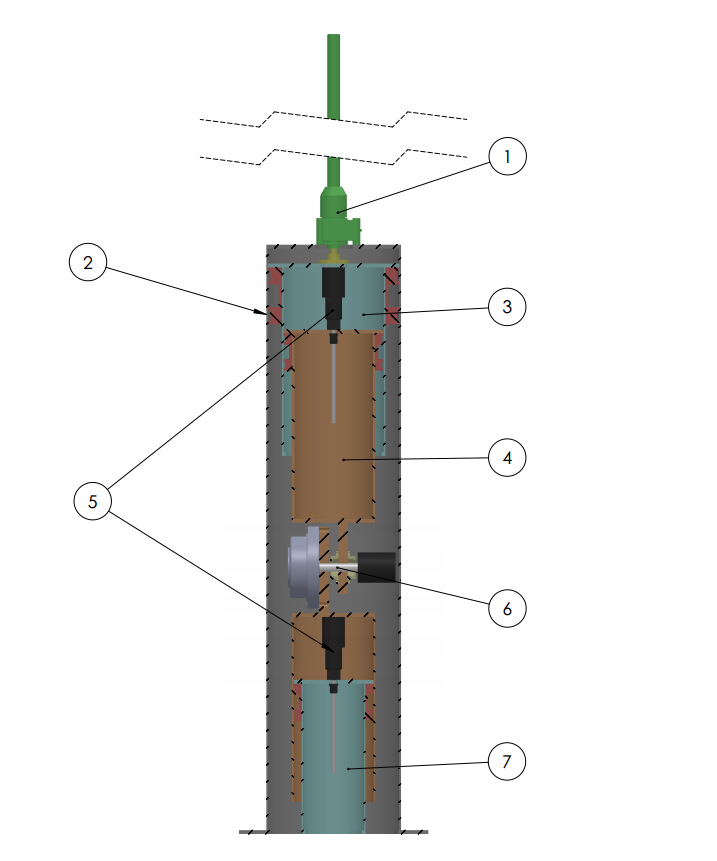
\includegraphics[width=\columnwidth]{figs/estudo/solid/Base_Recolhida.PNG} 
%	\caption{Initial configuration of the base (retracted)}
%	\label{fig::base_recolhida}
%\end{figure}

%\begin{figure}[h!]
%\centering
%	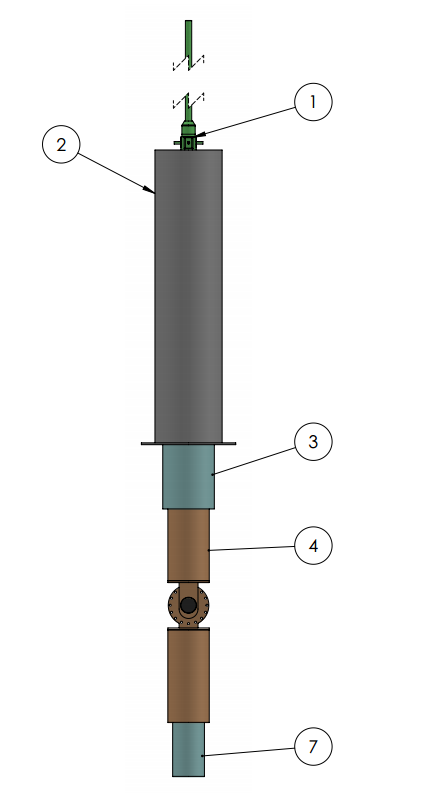
\includegraphics[width=\columnwidth]{figs/estudo/solid/Base_Extendida.PNG} 
%	\caption{Base on extended configuration}
%	\label{fig::base_extendida}
%\end{figure}

The main components of the base are shown in figure~\ref{fig::baselbr}: 1) worm
gear linear actuator; 2) fixed base; 3) prismatic arm \#1; 4) prismatic arm \#2;
5) linear actuators; 6) revolute joint; 7) prismatic arm \#3.
Figure~\ref{fig::base_ambiente3d_recolhida} shows the base and KUKA LBR R820 manipulator.

%Os componentes principais da base estão representados nas
%figuras~\ref{fig::base_recolhida} e~\ref{fig::base_extendida}, são: 1) atuador
%linear por sem-fim coroa; 2) base fixa; 3) braço prismático \#1; 4) braço
%prismático \#2; 5) atuadores lineares; 6) junta rotativa; 7) braço prismático
%\#3.

%A figura~\ref{fig::base_ambiente3d_recolhida} demonstra a base com o
%manipulador KUKA LBR 820 e as dimensões extremas, em milímetros, estimadas para
%% o interior e para fora da turbina, na configuração inicial de entrada no aro
%câmara pela escotilha superior.
%A figura~\ref{fig::base_ambiente3d_extendida} apresenta a base com o
% manipulador em uma configuração qualquer de operação, demonstrando o ganho de alcance e
%generalidade de posicionamento fornecidos pela base.

\begin{figure}[h!]
\centering
	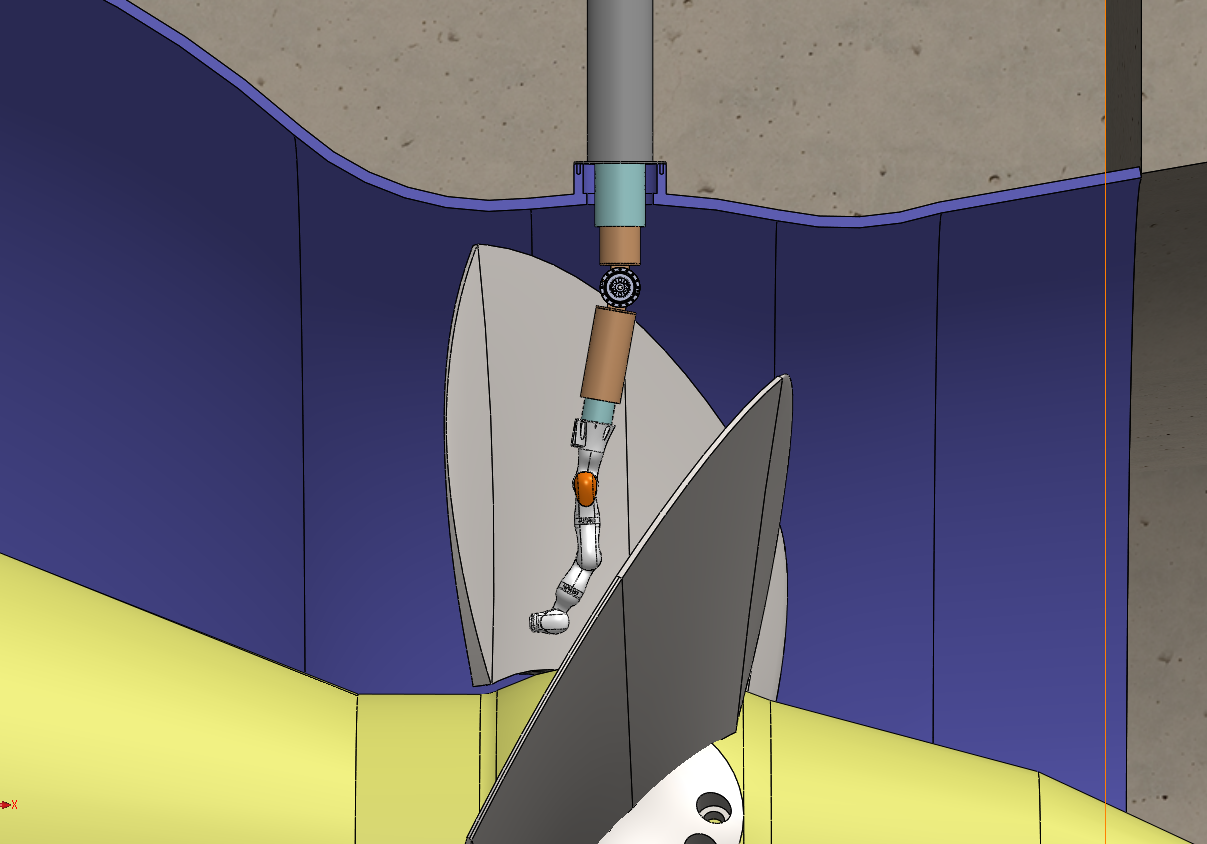
\includegraphics[width=\columnwidth]{figs/estudo/solid/Base_Ambiente3d_Operacao.PNG} 
	\caption{Base and KUKA LBR R820 manipulator}
	\label{fig::base_ambiente3d_recolhida}
\end{figure}

%\begin{figure}[h!]
%\centering
%
	% 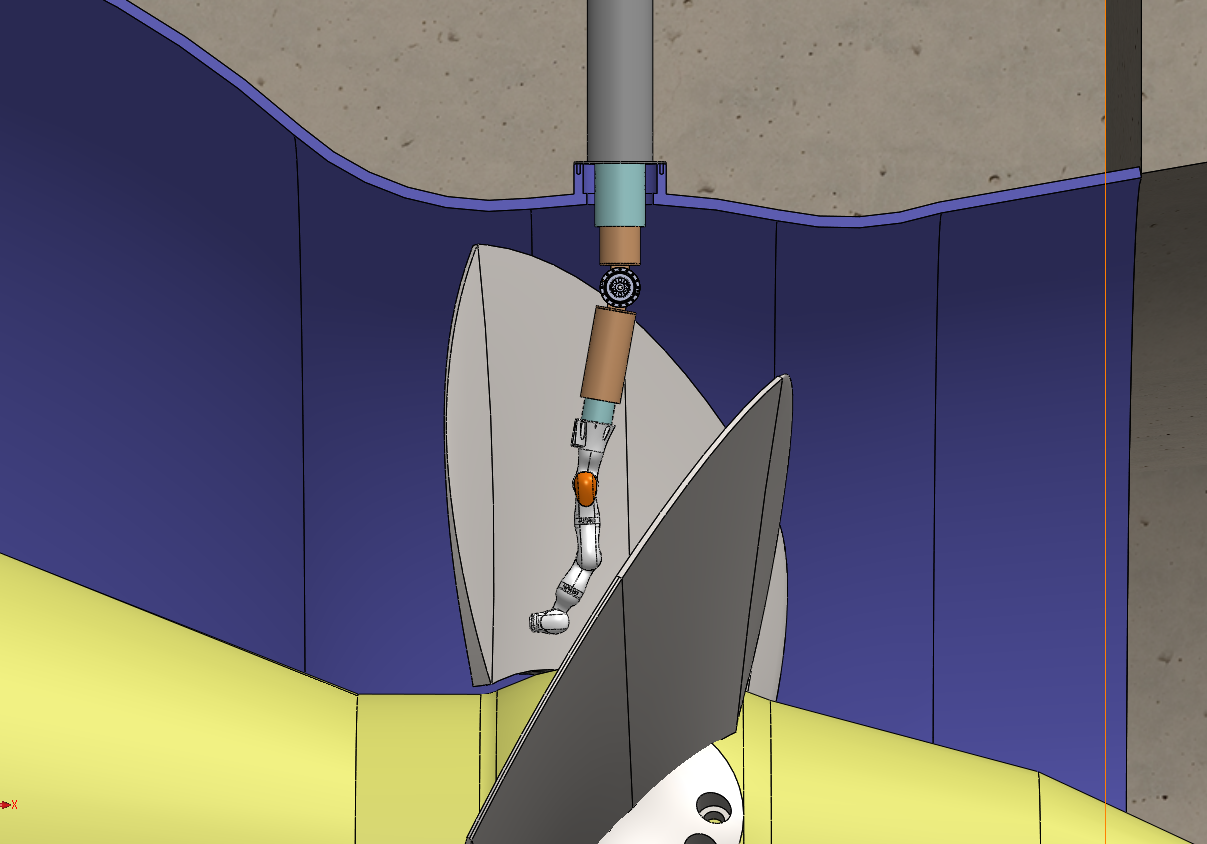
\includegraphics[width=\columnwidth]{figs/estudo/solid/Base_Ambiente3d_Operacao.PNG}
%	\caption{Base em uma geral configuração de operação}
%	\label{fig::base_ambiente3d_extendida}
%\end{figure}


%Tendo como objetivo posicionar o LBR R820 em uma posição onde seja capaz de
%trabalhar toda a pá, um modelo de base articulada foi proposto. A base
%composta de dois elos interligados por uma junta de rotação é fixada na
%própria escotilha. Para que seja possível cobrir toda a pá,
%a base deve ser capaz de assumir diversas angulações com respeito ao
%eixo de inserção, e a junta que conecta os dois segmentos da base também
% precisa ter sua posição alterada, o que pode ser realizado manualmente ou com atuador.

Inserting the system, composed of the base and manipulator, in the top
hatch, requires special care, as the system total length is greater
than the distance from the top of the arc chamber to the turbine nose. In
extended configuration, the arm and the base will need to be rotated during the
insertion process, which will result in system's central mass misalignment with respect to the
perpendicular axis of the hatch, thus it will require a guide to compensate
the generated torque.

%Introduzir o robô, composto pelo conjunto base-LBR R820, é uma tarefa cuidadosa
%pois a extensão total será maior que a distância do topo do aro câmara ao
%cone da turbina. Ou seja, o braço e a base precisarão ser rotacionados
%durante o processo de inserção, o que acarretará no desalinhamento do centro de
%massa (com relação ao eixo perpendicular à escotilha) e exigirá uma guia para
%resistir ao torque gerado por esse desalinhamento.


As the system is attached to the top hatch and the joint base is fixed,
the torques are expected to be less than 3000 Nm on joint base, and 4000 Nm on
the base during coating operation.

%Com o robô fixado na escotilha e a junta da base travada, são esperados torques
%inferiores a 3000 Nm sobre a junta e 4000 Nm sobre a base, durante a operação
% de revestimento.

%Ao se avaliar as possibilidades de realizar o revestimento sem a necessidade de
%placas de sacrifício, percebe-se que poderá ser realizado se a junta da
%base estiver paralela à pá (que para efeito de cálculo foi assumida com uma
%angulação de $45^o$ com relação ao eixo da turbina). Para esse caso a junta
% precisa realizar uma rotação à velcidade mínima de 34 rad/min. Essa velocidade possibilita a
%pistola de revestimento percorrer verticalmente a pá sem pausa. Percorrer
%horizontalmente a pá não será possível devido às restrições nas dimensções da
%base. O cálculo foi realizado por um estudo puramente geométrico, utilizando as
%informações reais de extensão da pá e área de trabalho do robô, assumindo um
%modelo simples da pá, sem curvatura.


\subsection{Bottom hatch}
The bottom hatch, localized at the bottom of the arc chamber, has 80 cm
diameter, enabling mid-sized robots entry, but it is 10 m far from the blade,
requiring system transportation and positioning. Using the bottom hatch as the
access for robot has the follwing advantages: large enough for medium sized
robots, free access, it is normally used by operators to turbine maintenance.
And the following disadvantages: not large enough for large robots, complex
logistics to the hatch (scaffolding and hoists), difficulty for robot moving
and positioning in the arc chamber due to the slippery and sloping floor.

%Solutions for the bottom hatch have the following advantages and
%disadvantages:
%Soluções que utilizem o acesso pela escotilha inferior, de dimensão maior,
%apresentam as seguintes vantagens e desvantagens:

%\textbf{Advantages}:
%\begin{itemize}
%  \item large enough for medium sized robots
%  \item free access
%  \item it is normally used by operators to turbine maintenance.
%\end{itemize}

%\textbf{Disadvantages}
%\begin{itemize}
%  \item not large enough for large robots
%  \item complex logistics to the hatch. Scaffolding and hoists are
%  needed
%  \item difficulty for robot moving and positioning in the arc chamber due to
%  the slippery and sloping floor.
%\end{itemize}

The bottom hatch, like all other accesses, is a logistical challenge and
a common challenge of the metallization process. The bottom hatch has 80 mm
diameter and is 4 m above ground. The system should be carried by a hoist
manually operated, installed inside the arc chamber on scaffolding. The floor
is slippery and has a cylindrical and inclined shape.

%O acesso pela escotilha inferior apresenta, como todos os outros
%acessos, um desafio logístico e o desafio comum do processo de metalização. O
%acesso à escotilha é realizado por uma abertura de 80 mm de diâmetro e 4 m
% acima do solo, logo os equipamentos são transportados por uma talha operada manualmente,
%instalada dentro do aro câmara, em andaimes. O solo é escorregadio e, devido à
%forma cilíndrica do aro câmara, curvilíneo e inclinado.

The system solutions were focused on medium size and lightweight manipulators,
due to robot shipping, handling and positioning of the robot. And modular base
solutions, when possible. Solutions were divided into subsections in accordance
with fixation strategies: mobile robots that move on rails fixed on the blade;
climbers; industrial manipulators that move on rails fixed on the floor.

%Dessa forma, as soluções foram focadas em robôs de médio porte, peso reduzido
%devido ao transporte e às necessidades de movimentação e posicionamento do robô
%(trajeto escotilha à pá), e modular, quando possível.

%As soluções foram divididas em subseções de acordo com a fixação:
%robôs móveis que se locomovem em trilhos, robôs escaladores e manipuladores
%industriais com base fixa. 
%obs.:
%Colocar o robô entre as pás para aplicar revestimento de duas pás com uma
% instalação exige que o robô seja desmontado toda vez que a turbina for girada.
%Isso é ruim, pois após primeira aplicação a área fica de risco. Esta solução
%exige 5 movimentos no robô e 6 movimentos na turbina.

%A solução em que o robô fica atrás ou à frente exige que o robô seja
%movimentado apenas 2 vezes e a turbina fará 8 movimentos (duas voltas).

%TODO revisar todos os projetos sabendo as respostas
\subsubsection{Design of a mobile robot and rail fixed on blade}\label{proj_rail}
The concept solution of a robotic manipulator and rail base fixed on blade
satisfies all requirements for the HVOF coating and the inspection process. The
development of a compact system for easy transportation and its installation on the arc
chamber are possible, since the manipulator dimensions are reduced due to the
extra mobility provided by the rail.

%A utlização de um manipulador robótico sobre trilhos satisfaz todos os
%requisitos para a realização de um processo de inspeção e metalização
%utilizando a técnica HVOF. O desenvolvimento de um sistema compacto para o
%transporte através do acesso pela escotilha inferior e sua instalação no aro
%câmara da turbina são possíveis, pois as dimensões do manipulador podem ser
%reduzidas por meio da mobilidade extra proporcionada pela introdução do trilho.

In the context of the proposed application, the solution consists in a system
similar to Roboturb, presented in section \ref{sec::rail}. Thus the rail should
be flexible to be able to follow the blade curvature, it should allow several
placement options, and, as the blade is not ferromagnetic, the adhesion would
be by active suction cups with special material to work on large temperature
variations.

%No contexto da aplicação proposta, foram concebidas duas possibilidades para a
%fixação do sistema de trilhos. A primeira solução consiste em um sistema
%semelhante ao Roboturb, apresentado na seção \ref{sec::rail}. O sistema
% proposto se trata de um manipulador robótico com fixação diretamente na pá da
%turbina. O trilho deverá ser flexível para ser capaz de acompanhar a curvatura
%da pá e possibilitar diversas opções de posicionamento. Como o material da pá
%não possui alta permeabilidade magnética (Inox 420), a solução de fixação seria
%por ventosas ativas e com material específico para suportar as grandes
%variações de temperatura que a pá pode alcançar (temperatura ambiente a
%$100^oC$ durante a metalização).

%Uma abrangente pesquisa de robôs comerciais industriais de pequeno porte
% apontou que há manipuladores com carga entre 12 e 20 kg e velocidade necessários,
%sendo o LBR da Kuka o que possui melhor benefício peso/alcance, 30 Kg e 820 mm,
%respectivamente. %Para este manipulador, a metalização deverá ser
%realizada em, pelo menos, quatro etapas com quatro trilhos diferentes e
%customizados, e placas de sacrifício para evitar mau aplicação da metalização
%durante as trocas de sentido na movimentação do robô.

%A fixação de um trilho na pá apresenta diversas complexidades, como: a
%necessidade de manualmente instalar/desinstalar o sistema trilho/robô diversas
%vezes em cada pá; o projeto do trilho customizado e flexível; e ventosas ativas
%especiais que suportam variação de temperatura.




\textbf{Solution conclusion}

Fixing a rail on the blade has some complexities: rail and robot manual
installation/uninstallation for each blade side; design of customized flexible
rail; and design of special active suction cups for high temperature
variation. It is possible to use an industrial manipulator, such as the
Kuka lightweight (30 kg), making the design focused on signal processing,
mapping, localization, control, and the rail construction. 

%A solução com trilho externo se mostrou vantajosa em comparação ao robô em
%trilho customizado acoplado à pá, devido à complexidade e intervenções
%manuais. Há a possibilidade de utilizar um manipulador industrial, tornando o
%foco do projeto em processamento de sinais, mapeamento, localização e controle,
%além da construção do trilho. Porém, a montagem da estrutura e a instalação de
%todo o sistema atrás da pá podem ser custosas, sendo esta ainda uma solução
%considerada complexa.
\subsubsection{Design of robotic climbers}\label{proj_climbers}
In this subsection, the robotic solutions for HVOF coating are the fusion
of technologies documented in subsection~\ref{sota_climbers}. They will be an
adaptation of \emph{The Climber}, ICM, given their ability to reconfiguration.

%Nesta subseção, consideram-se soluções para HVOF de pás de turbinas robôs
%escaladores com fusão das tecnologias documentadas na
%seção~\ref{sota}, subseção~\ref{sota_climbers}. Será abordada uma versão
%adaptada do robô \emph{The Climber}, ICM, dado sua possibilidade de
%reconfiguração.

\emph{The Climber}, ICM, is a commercial solution which meets many
of the HVOF specifications and enables improvement without compromising its
structure. The robot's adhesion is suction type and the motion is flexible
mats.
The system has already been tested in hazardous environments, as wind turbines,
hydroelectric plants and others. We can divide the design into four systems:
mobility, adhesion, manipulator and autonomy.

%O robô \emph{The Climber}, ICM, é uma solução comercial que atende muitas das
%especificações HVOF e possibilita aperfeiçoamento sem comprometer sua
%estrutura. O robô possui sistema de adesão por sucção e locomoção através de
%esteiras flexíveis. O sistema já foi testado em ambientes de alta
%periculosidade, como turbinas eólicas, usinas hidrelétricas e outros. Podemos
%dividir o projeto em quatro sistemas: locomoção, adesão, manipulador e
% autonomia.

\emph{The Climber} uses only one vacuum chamber instead of the suction cups in
\cite{kim2008development}, for example. \emph{The Climber}'s flexible mats allow
smoothly and continuously motion. The solution with a single chamber seems more
advantageous, as the robot can move on curvatures up to 30 cm radius.

%O sistema desenvolvido em \cite{kim2008development} tem mecanismo de
%locomoção por esteiras e adesão por sucção. O sistema é composto por polias,
%correias de borracha, ventosas, válvulas para cada ventosa, motores DC para as
% polias, sistemas de controle para as válvulas e para os motores. \emph{The Climber}
%utiliza apenas uma câmara de vácuo, em vez de ventosas, e esteiras flexíveis
% que permitem maior suavidade e continuidade ao movimento. A solução por uma única
%câmara parece mais vantajosa, já que o robô consegue se locomover em curvaturas
%de até 30 cm de raio.

In the specific case of the HVOF process, a manipulator applies the coating 
while the robot travels along the blade. The robot locomotion on the blade rises
some design issues: the blade temperature during the procedure requires an
active suction chamber special material; and mats and suction chamber must
work on highly curved surface.

%No caso específico da aplicação HVOF, o processo é realizado com
%manipulador enquanto o robô percorre a pá da turbina. A locomoção do
%robô sob a pá levanta algumas questões de projeto: a
%temperatura da turbina durante o procedimento exige uma solução por câmara
% ativa de material especial; e como se comporta o robô em curvaturas
%acentuadas. 


In adhesion by suction, an intelligent security mechanism should be implemented,
with accelerometers, gyros and other sensors to ensure the shutdown of the
electronics and the supply of the HVOF gases in case of fall. The solution of a
mobile robot path planning increases safe operation and the optimal control of the adhesion
mechanism can limit the maximum suction force.

%Em sistemas de adesão por sucção, deve-se considerar um mecanismo
%inteligente de segurança, possivelmente utilizando acelerômetros e outros
%sensores, para garantir o desligamento do sistema eletrônico e o fornecimento
% de gáses. A solução de um robô móvel com planejamento de trajetória aumenta a
%segurança da operação e o controle ótimo do mecanismo de adesão pode limitar a
% força máxima de sucção.


%O manipulador a ser projetado para aplicação HVOF possui as seguintes
%características: é leve para não comprometer a adesão e equilíbrio do sistema
%móvel; rápido e preciso conforme requer a aplicação HVOF; modular, já
%que a operação será realizada in-situ, em espaço confinado;
%não possui grandes dimensões, pois o robô é móvel e pode
%percorrer a pá, porém deve ser suficiente para operar em pontos de
%difícil acesso à base e considerar a distância mínima (230 mm) entre pistola
%HVOF e pá; e é capaz de sustentar a carga e vibrações geradas pela
%pistola HVOF. 

% Climber's path planning solution should consider both the mobile base and the
% manipulator. The literature is fairly consolidated on robotic manipulators, and
% many of these problems are already settled and available, as developed in
% \cite{manzdevelopment}. 

%A solução de robôs escaladores exige planejamento de trajetórias tanto da base
%móvel, quanto ao controle de manipuladores. A literatura sobre
%manipuladores é bastante consolidada, sendo muitos dos problemas citados já
%resolvidos e disponíveis no mercado, como o desenvolvido em
%\cite{manzdevelopment}. Os menores manipuladores industriais que sustentam a
%carga do sistema de metalização possuem em torno de 30 a 50 kg. Portanto, o
%conjunto manipulador, pistola e cabos pode possuir de 50 a 80 kg de massa.

%A tecnologia que verifica a necessidade de
%revestimento, com sensores laser e ultrassom, e poderá indicar o \textbf{mapa
%ou apenas realizar um teste de sucesso/falha} \citep{escaler2006detection}.

% The mission control is the planning and execution of tasks. The motion and
% adhesion control should be synchronized, performing the path planning,
% obstacle avoidance and environmental mapping, through a set of sensors such as
% accelerometers and laser. The manipulator control can be kinematic by visual
% servoing or by structured environment. And a vehicle support system will be
% responsible for security, smooth operation and power management.

%O sistema autônomo de um robô móvel é a inteligência do robô. Ele abrange o
%controle de missão, ou seja, o planejamento e execução das tarefas em modo
%autônomo. A locomoção será realizada pelo controle dos motores em conjunto com
% o controle do sistema ativo de adesão por sucção, o planejamento de trajetória, desvio de
%obstáculos e mapeamento do ambiente, através de um conjunto de sensores, como
%laser e acelerômetros. O controle do manipulador poderá ser cinemático por
%servovisão ou pela estruturação do ambiente. E um sistema de suporte do veículo
%ficará responsável pela segurança, bom funcionamento e gerenciamento de
% potência do robô.




%As características descritas acima como solução de um robô escalador impede a
%troca automática entre pás. Um robô escalador com tecnologia de avanço
% pendurado por braços é uma solução muito custosa em termos de controle e estrutura
%mecânica. Outra solução seria um robô com locomoção por segmentos deslizantes,
%como o RRX3, e adesão por sucção, porém a flexibilidade exigida para a
% locomoção entre pás e a distância entre turbinas complexifica o projeto. Dessa forma, a
%troca entre pás deverá ser manual.

%\textbf{Versão adaptada Roboturb}

%O Roboturb, como já descrito na subseção~\ref{sec::rail}, é um
%manipulador que se locomove em um trilho, este acoplado à pá da turbina
%por ventosas (sucção). A solução não permite a extensão
%do manipulador, já que o peso desequilibra a estrutura e não há torque para
%compensar a força exercida no efetuador durante a operação HVOF. A segunda
%solução de robôs escaladores é adicionar um trilho perpendicular e transformar
%o Roboturb em um robô móvel, com locomoção através de dois trilhos, idéia
%semelhante ao \emph{Climbing robot for Grit Blasting}, que utiliza duas
%plataformas deslizantes com ventosas.

%Os trilhos são compostos por esteiras flexíveis nas extremidades para a
%locomoção, como \emph{The Climber}, e as ventosas são ativas e distribuídas por
%todo o trilho. O manipulador só necessitaria mover em um dos trilhos para
%percorrer toda a pá, já que os trilhos também se movimentam. 

%A solução de trilhos móveis com manipulador é dependente à curvatura da pá da
%turbina e o aumento da flexibilidade do trilho para se locomover sob a pá pode
%impedir a movimentação do manipulador. Dessa forma, é considerada uma solução
%muito específica e restrita à aplicação.

\paragraph{Solution conclusion}
Although tempting because of the autonomy, the surface complexity of the
turbine blade, the confined environment, and the required speed and payload are
major challenges to the design. 

The climber's manipulator would be complex and should have the
following characteristics: to be lightweight, avoiding base complex adhesion and
balance; to be fast and accurate as required by the HVOF application; to be
modular, as the operation is performed in confined spaces; to
be small, improving mobility, but capable to operate on blade's edges with 230
mm minimum distance; and to have high payload and vibration resistance. The
smaller industrial manipulators with required the payload weighs 30 to 50 kg.
Therefore, manipulator, HVOF gun and cables weighs 50 to 80 kg. The
manipulator greatly increases the dimensions of the mobile base and hence
diminishes their workspace, slowing the process.

Finally, the climber as described above does not switch automatically between
blades. A climber with arms to switch between blades is a costly solution in
terms of control and mechanical structure. Another solution would be a robot with
locomotion by sliding segments, as RRX3, and adhesion by suction, but the
flexibility required for motion between blades complicates the design. Thus,
the exchange between blades should be manual.

Compared to alternative solutions, a climber would be a general solution,
it has logistical advantages, but it is a robotic challenge. 

%Apesar de tentador devido à autonomia, a complexidade da estrutura da pá, o
%ambiente, a velocidade requerida e a carga do sistema de metalização são
%grandes desafios ao projeto. São estimados 50 kg de
%carga para o conjunto manipulador, cabos e pistola, o que aumenta muito as
%dimensões da base móvel e, consequentemente, diminui a sua área de atuação,
%tornando o processo mais demorado.
\subsubsection{Proposed solution}\label{proj_manip}

There are several industrial manipulators which fulfill the HVOF
requirements. Companies as Fanuc, Motoman, ABB and KUKA, for example,
manufacture manipulators compatible with the bottom hatch dimensions and HVOF
requirements, and workspace that the entire turbine blade could be coated at a
fixed base position. However, those manipulators are too big to operate behind
the blade, on the distributor side, due to environment collision, joint
constraints, and robot manipulability. Besides, manipulators with such
workspace are heavyweight, thus the robot placement and motion would be complex
inside the Runner area. A feasible solution would be to select a mid-sized
manipulator and made a rail base to place and move the robot.

%Há diversos manipuladores robóticos industriais com as especificações
%necessárias para a realização da tarefa de metalização por HVOF. As empresas
%Fanuc, Motoman, ABB e KUKA fabricam manipuladores com dimensões compatíveis com
% o acesso pela escotilha inferior e velocidade, precisão, e espaço de trabalho que
%cumprem os requisitos para a execução do processo em todo um lado da pá, em uma
%base fixa. Porém, há incompatibilidade atrás da pá e a necessidade de escolher
% a posição correta do manipulador em relação à pá, a fim de maximizar a sua área de trabalho, no ambiente da
%turbina, o que pode restringir os seus movimentos.
%Como as pás podem ser giradas até um ângulo de $14.5^o$, são discutidas as
% ideias de posicionamento do manipulador entre as pás, a fim de executar a operação em ambos os lados da
%pá (um lado de cada pá), e o posicionamento fixo à frente e depois atrás à pá.

The base consists of a transport rail and a positioning rail, both fixed
in the Runner area by magnetic coupling and/or welding. The first solves a
logistic problem, as it starts at the bottom hatch entry and goes to the blade,
moving the robot through the Runner area. The latter is coupled to the main rail and positions the robot close to the
blade, enabling displacement along it, solving the horizontal HVOF cover of the
blade.

The base may be summarized in three joints: prismatic (main rail), revolution
(joint between main and second rail), and prismatic (second rail) (P-R-P). As
the robot can not vertically cover the entire blade, there is still the need of
different vertical positions, which should be manually selected. The blade can
be coated on linear or circular motion, and, in both cases, the manipulator will
be responsible for speed, position and gun orientation. The solution for gun
direction exchange (\textit{long stop}) is an actuated valve to redirect the
coating particles.

%A base por um trilho de transporte e um de posicionamento. Ambos são fixados no
%aro câmara por acoplamentos magnéticos e/ou solda. O primeiro começa na
%entrada da pá e vai até a pá, permitindo o deslocamento do robô pelo aro
% câmara.
%O último é acoplado ao trilho principal e posiciona o robô próximo a pá, além
% de possibilitar o deslocamento ao longo desta. Dessa forma, a base pode ser
%resumida em três juntas: prismática, revolução e prismática (PRP). Como o robô
%não possui alcance de toda a pá, há, ainda, a necessidade de posições verticais
%diferentes escolhidas manualmente. A pá pode ser processada em movimentos
%circulares ou lineares e, em ambos os casos, o manipulador ficará responsável
% pela velocidade, posição e orientação do processo. A troca de sentido de movimento deverá ocorrer fora da
%pá, ou devem ser utilizadas placas de sacrifício, ou válvulas para
%redirecionamento das partículas de revestimento.

%Esse tipo de abordagem simplifica a movimentação do robô no
%trilho, uma vez que o trilho seria totalmente reto, e possibilitaria a
%metalização de um dos lados das quatro pás com uma única instalação de base.
%Porém, mesmo nesta solução, a altura do trilho deverá ser ajustada três vezes
% para cada lado de pá.


%Em ambos os sistemas propostos, é necessária a implementação de um sistema de
%localização do robô em relação à pá, tornando possível a geração de um
%planejamento de trajetórias para o processo de metalização. O sistema de
%localização pode ser concebido por sensores externos
%ao robô (câmeras e outros), ou instalados no próprio manipulador/base.


%The alternative to avoid contact with the blade consists of a single rail
%rectilinear fixed by magnetic bases or welding of the rim in the soil chamber.
% Like the robot has not reach all the shovel, there is still a need positions
%different vertical. The blade can be processed in circular movements or
%linear and, in both cases, the handler will be responsible for the speed,
%position and orientation of the process. The exchange direction of movement
% should occur outside the shovel or must sacrifice cards used.

%\paragraph{Transport rail}

A mid-sized robot manipulator should be hoisted through the bottom
hatch, placed on a rail base with magnetic holders and carried
to the blade, as in Fig.~\ref{fig::rail1}. At that position, the robot should
switch to the other rail. 
%That strategic position (robot between blades) is
% advantageous as it allows the manipulator to operate adjacent blades without
% rail disassembling or major positioning changes.

\begin{figure}[h!]	
	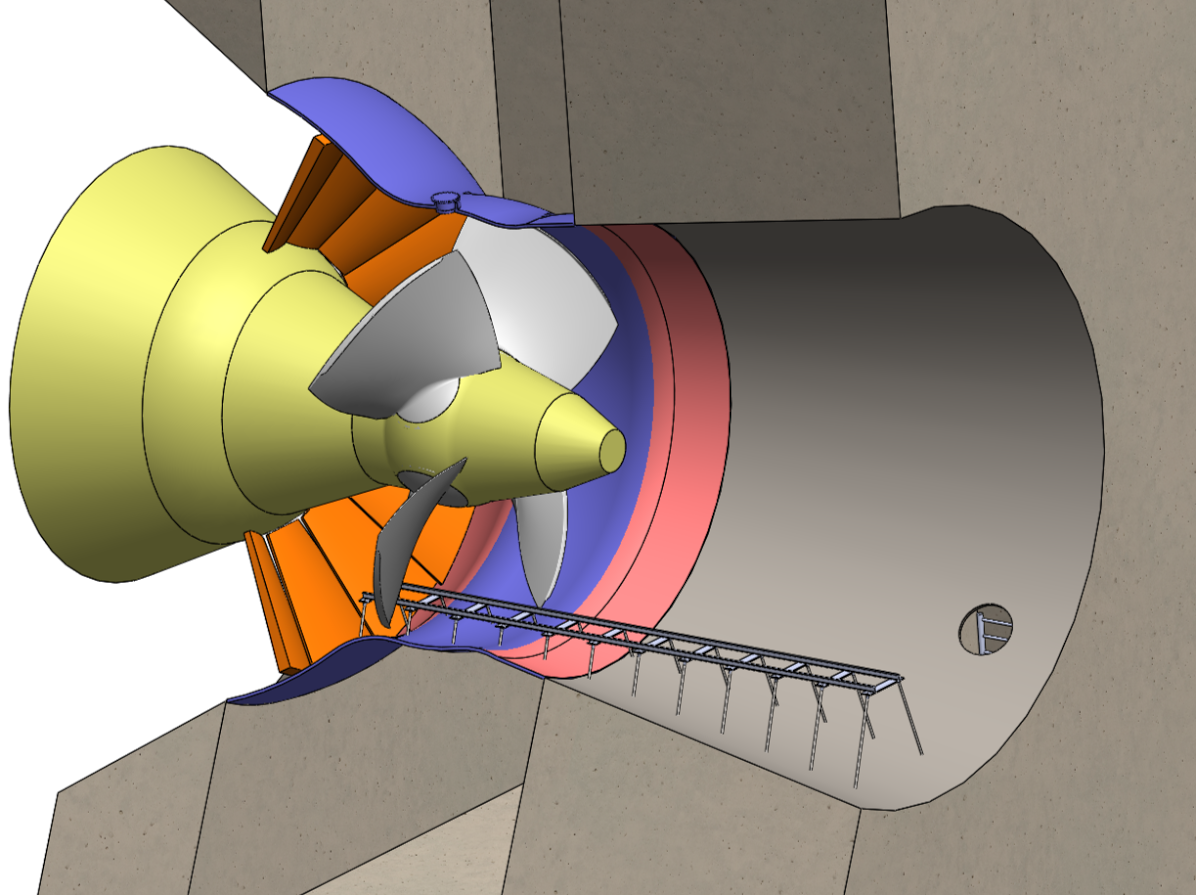
\includegraphics[width=\columnwidth]{figs/manipuladores/rail1.PNG}
	\caption{Transport rail mounted inside the turbine.}
	\label{fig::rail1}
\end{figure}

%A figura~\ref{fig::andaime} mostra o espaço entre as pás da turbina, dentro do
%aro câmara. Um robô manipulador de médio porte pode ser fixado em uma base
%magnética, na posição que se encontra a escada da figura~\ref{fig::andaime}.
%Essa posição é vantajosa por possibilitar a execução da tarefa em duas pás
%(frente de uma e verso da outra), sem desmontar ou fazer grandes alterações no
%posicionamento da base do robô, diminuindo as intervenções e tempo de tarefa.

% However, a purely geometric study shows that the necessary workspace for
% adjacent blades coating, assuming a fixed base between the blades,
% is around 5 m reach. The industrial manipulator IRB5500, for example, developed
% by ABB for painting, and is a large sized manipulator and has 3 meters range,
% 600 kg.
% As no mid-sized industrial robot was found for completely cover
% the blade on a fixed base position, a positioning rail should be made.

%O estudo puramente geométrico demonstra que o alcance do manipulador robótico
%para o processamento de ambos os lados das pás, considerando uma base fixa
% entre as pás, deverá ser em torno de 5 metros. O manipulador industrial IRB5500,
%desenvolvido pela ABB para pintura, possui 3 metros de alcance, porém 180 kg, o
% que já dificulta ou até impossibilita a logística de movimentação e posicionamento in-situ. Não foi encontrado um robô
%industrial com o alcance necessário e que tivesse as dimensões máximas da
%escotilha inferior. 

%A solução conceitual de posicionar um manipulador industrial entre as pás deve
%avaliar, portanto, todas as configurações necessárias da base (orientações e
%posições) para garantir que todo o espaço de trabalho do manipulador mais base
%cubra os lados de ambas as pás. O número de configurações e o projeto
%mecânico da base são necessários para a viabilização da solução,
%uma vez que será possível avaliar as intervenções e complexidades. Bases
%autônomas diminuem o número de intervenções e aumentam a precisção do sistema,
%porém aumentam a complexidade, o custo devido ao número de sensores e
% atuadores, e o peso do sistema, prejudicando a logística.

%\paragraph{Positioning rail}
Fixedly positioning a robotic manipulator with magnetic holders at the front or
at the back of the blade for HVOF process is a natural solution, since it is
similar to the companies procedure. However, a purely geometric
study, using the real dimensions of the blade, shows that the manipulator must
have more than 2.5 m reach for full blade cover. To perform this task, workspace
analysis was conducted to confirm the geometric study and a mid-sized
robot can not reach the entire blade. Therefore, its base should be able to move
horizontally and vertically (Fig.~\ref{fig::rail2}).

\begin{figure}[h!]	
	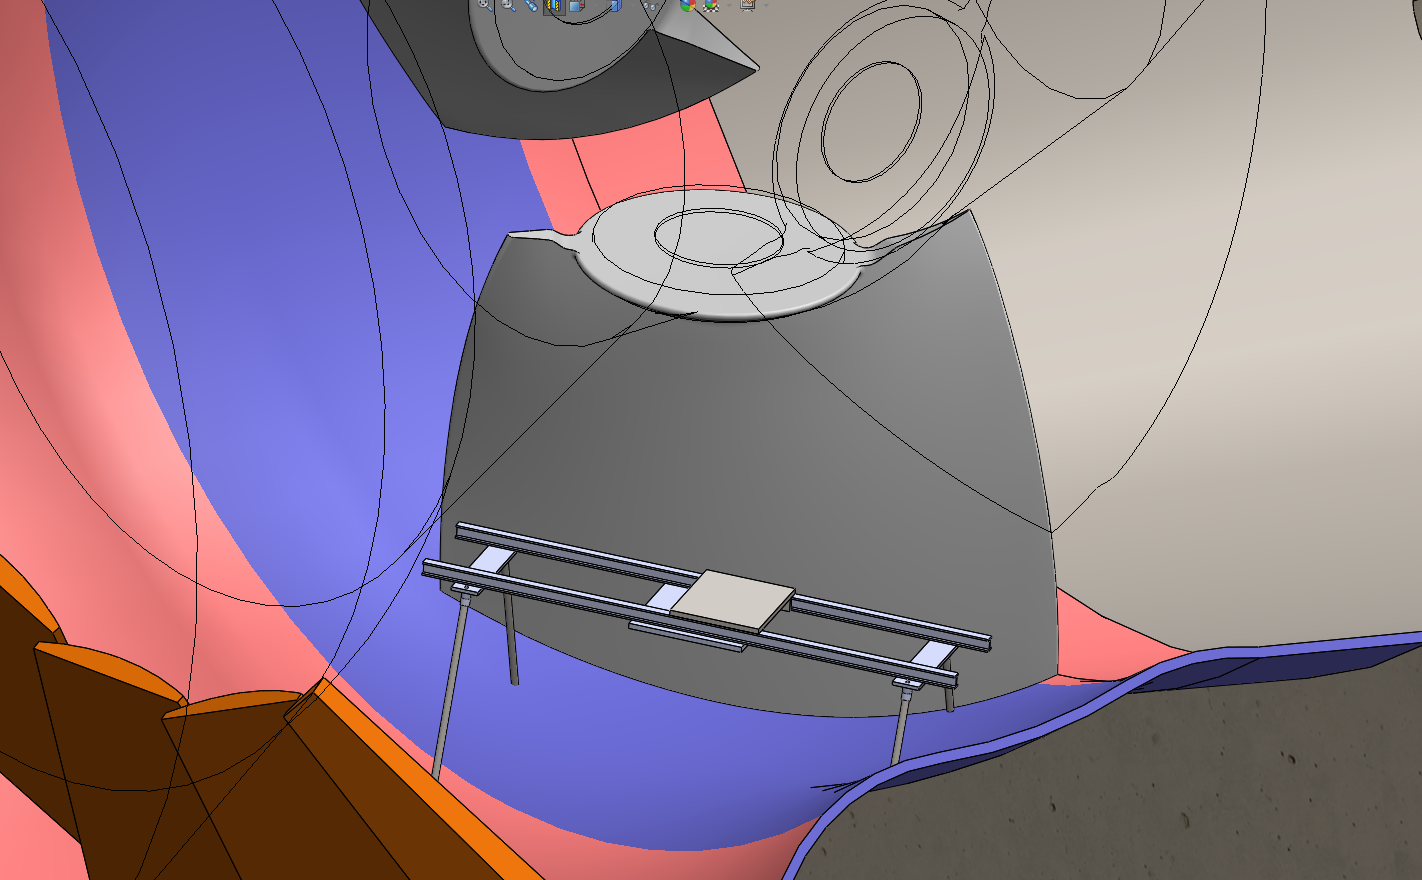
\includegraphics[width=\columnwidth]{figs/manipuladores/rail2.PNG}
	\caption{Positioning rail behind the blade.}
	\label{fig::rail2}
\end{figure}
%Posicionar de maneira fixa um manipulador com base magnética à frente e atrás
% da pá para a metalização é uma solução natural, já que é semelhante à utilizada pela
%empresa Rijeza atualmente. Um estudo puramente geométrico, utilizando as
%dimensões da pá, mostra que o manipulador deve possuir alcance de 1.7 m e ser
%posicionado a uma altura de 1.1 m em relação ao solo. Estudos de espaço de
%trabalho, manipulabilidade e colisões devem ser realizados para confirmar o
%estudo geométrico.

This design also requires the implementation of a localization/calibration
system, as the robot must know its location in relation to the blade for
autonomous operation. The localization requires external sensors, as cameras, a
3D laser for mapping, a point laser sensor installed on the manipulator's
end effector, and base odometry for position feedback.

In this solution, a robot placed on a rail type base, on the floor, can not coat
the blades on top, thus the turbine must be manually rotated and a new
calibration process should be done for each step.

%O posicionamento do sistema à frente ou atrás da pá exige
%intervenções para rotação da turbina e para o deslocamento do sistema. Em
% relação a um sistema com base autônoma entre as pás, o processo parece mais custoso em
%intervenções manuais e mais demorado, porém bem mais simples em termos de
%robótica.

\paragraph{Solution conclusion}
In terms of robotics, industrial manipulators on a rail base is the simplest
among all solutions for the bottom hatch. There is no mechanical design for the
manipulator, since it will be acquired in one of the aforementioned
manufacturers, but the mechanics will be responsible for the base design (rigid
and modular), the magnetic couplings, and logistics.

%In
%addition, the following steps should be done:
%manipulator control, data processing, calibration, path planning and UI.

%A utilização de manipuladores industriais é a mais simples, em termos de
%sistemas robóticos, dentre todas as soluções para o acesso pela escotilha
%inferior.

%Não há projeto mecânico do manipulador, já que este será adquirido em um dos
% fabricantes citados. As dificuldades mecânicas do projeto serão em relação à logística de posicionamento e movimentação do robô dentro do aro câmara, e no desenvolvimento de uma base,
%que pode ser autônoma. Além disso, o projeto fica responsável pelo controle do
%manipulador, processamento de dados que envolvem o HVOF, planejamento de
%trajetórias e UI.

%The main challenge is to build a rigid base and the locomotion of
%Equipment for the ring chamber. This conceptual design will be one of fronts to
%the feasibility study.

%Os desafios consistem na construção de uma base rígida e a locomoção dos
%equipamentos pelo aro câmara. Este projeto conceitual será uma das frentes para
%o estudo de viabilidade.
 
%% TODO Elael: Nosso projeto cabeado
\subsubsection{Robô Bipartido}

Esse conceito é uma cadeia de dois manipuladores conectados por um ponto de
apoio capaz de fixar-se à pá. O apoio serve como forma reduzir o torque
necessário nas juntas ao reduzir a alcance necessário para cada manipulador
individualmente.

Para facilitar futuras referências nesse texto, o braço robótico que se
apoia sobre o chão será chamado de primário, manipulador que parte dele de
secundário e o ponto de apoio entre eles, capaz de fixa-se à pá, será chamado de
fixador.

A pistola de metalização presa ao manipulador secundário deve ter
alcance sobre toda a pá da turbina. Para isso existe uma gama de pontos
necessários onde o fixador deve ser posicionado. Com esse intuito o
manipulador primário da cadeia precisa ser projetado para ter uma região de
trabalho com um alcance total sobre esses pontos. Para tal, informações precisas
sobre o formato das pás são necessárias.

Para viabilizar a solução, é necessário verificar quais são as soluções
possíveis para gerar a aderencia do fixador sobre à pá. As tecnologias mais
difundidas são por força magnética e por diferença de pressão (ventosa).
As maiores preocupações com o relação a adesão são a capacidade de carga do
método e a resistência do \textit{coating}. As soluções por magnetismo e
por ventosa afetam de maneira diferente as camadas do material ao qual se
aderem. Enquanto o magnetismo atrai ativamente o material ao qual prentende
aderir, a ventosa apenas reduz a pressão do ar na região onde ela se fixa. Ambas
as soluções possuem versões ativas e passivas, assim como uma gama de opções com
relação à capacidade de suportar carga. Logo, para essas soluções, a carga
necessária a ser suportada, o magnetismo do material, a resistência à baixa
pressão do \textit{coating} e os efeitos da atração magnética, também, sobre o
\textit{coating} são perguntas que devem ser respondidas.

O braço secundário deve ser projetado para atingir os requerimentos de
posicionamento e velocidade da pistola de metalização, porém a região sob o
fixador, certamente, não estará disponivel para receber o revestimento. Assim, a
possibilidade, ou os requisitos necessários, de mover o fixador para uma região
da pá recém metalizada deve ser vista analisada antes do robô bipartido ser
considerado uma possibilidade.

\subsection{Robô Pendurado} 

%\subsection{Acesso pela jusante}
Como última opção de acesso ao rotor, existe a possibilidade de utilização do
tubo de sucção ou descarga como meio de entrada à turbina. Com o fluxo de água
parado, é possível utilizar o Rio como meio de lançamento do sistema. A
complexidade da operação para utilizar esse acesso é maior, entretanto existem
vantagens que podem tornar essa solução viável e mais atrativa.

\textbf{Vantagens}
\begin{itemize}
  \item Virtualmente nenhuma restrição de tamanho
  \item Flexibilidade de soluções
  \item Facilidade de utilização de um manipulador industrial padrão
  \item Possibilidade de implementação em outras usinas
\end{itemize}

\textbf{Desvantagens}
\begin{itemize}
  \item Complexidade de lançamento e recuperação
  \item Custo
  \item Possibilidade de correnteza
  \item Complexidade logística de transporte entre a entrada do tubo de sucção e
  o aro câmara
  \item Complexidade de prototipação
\end{itemize}

As soluções foram divididas em etapas necessárias para a operação, ou
seja, lançamento e recuperação do sistema, logística de transporte e o robô de
metalização propriamente dito.

Para esse acesso, o maior obstáculo presente é o desenvolvimento de um sistema
de lançamento e recuperação do robô, a partir do rio, até o interior da turbina.
Essa operação deverá ser realizada com a turbina alagada e, em seguida,
pode-se dar início ao processo de drenagem da
mesma.
É importante que o sistema de lançamento seja robusto e garanta o perfeito posicionamento do robô dentro da turbina, assim
como, a sua recuperação, uma vez que erros nesse processo podem significar a
perda completa do sistema.

Primeiramente, a solução deve ser a prova d'água com classificação para pelo
menos 50m de profundidade.
Sendo assim, um vaso de pressão para o transporte do robô até o interior da turbina deve ser
desenvolvido, não havendo necessidade do maniupulador responsável pela
metalização ser a prova d'água. O \textit{container} de transporte
submarino deve ser menor que o tamanho do vão do stoplog, visto que o acesso
mais próximo ao tubo de descarga, pelo rio, se dá por esse vão.
Por outro lado, suas dimensões devem ter um tamanho mínimo que possibilite o
encapsulamento do robô e todo o material de suporte necessário. Há aindaa
necessidade de uma escotilha de acesso de tamanho suficiente para que todo o
sistema seja retirado do interior do \textit{container} submarino.

Para o sistema de lançamento, foi deslumbrada uma estrutura de transporte que
utilizará o pórtico rolante e o trilho guia dos stoplogs. Após a submersão da
estrutura, um mecanismo de lançamento, inspirado em um paletizador, é
responsável pelo posicionamento do \textit{container}, sempre no mesmo ponto em
relação ao tubo de descarga. Com o vaso de pressão posicionado, a turbina deve
ser, então, drenada. Em seguida, o robô pode ser retirado de seu
envólucro e a operação de metalização pode ter seu início. Uma etapa crítica da
operação é a recuperação do sistema, na qual a turbina deve ser novamente
alagada e os os stoplogs retirados. A estrutura de transporte deve, então,
recuperar o \textit{container} transportador na mesma posição em que o sistema
foi lançado. O sucesso dessa operação tem como \textbf{hipótese que a velocidade
de drenagem e a correnteza gerada por essa operação não são suficientes para
retirar o container (mais pesado que a água) de sua posição inicial}. 

A movimentação do robô do ponto de lançamento até o aro câmara deverá ser
realizada a partir da utilização de cordas, roldanas e talhas. Caso necessário,
pode ser desenvolvido um sistema de locomoção com trilhos e/ou rodas atuadas
para o posicionamento automático do robô e, até mesmo, um plano elevado para
transporte.

O robô de metalização pode ter diversos fomatos, mas devido a possilidade de se
utilizar um manipulador industrial padrão, o projeto inicial consiste em uma
base de apoio e um manipulador com alcance para o processamento de uma face da
pá posicionado de frente para pá, ou um manipulador posicionado entre duas pás com
alcance para processar as duas as faces das pás voltadas para ele.













\subsection{Conceptual solution}
As a conclusion of the proposals, the concept solution is to use an
industrial manipulator on a customized base. The characteristic of the
manipulator and the base varie with the hatch (top or bottom). If top hatch, the solution is a small
sized industrial manipulator and custom telescopic base, electronically
operated; in the case of the bottom hatch, the solution is a mid-sized industrial manipulator
with rail type bases and magnetic holders.

%Como conclusão das propostas, a solução conceito é a utilização de um
%manipulador industrial sobre uma base. A característica do manipulador e da
% base varia de acordo com o ponto de acesso: no caso
%da escotilha superior, a solução é um manipulador industrial de pequeno porte e
%base customizada operada eletronicamente; no caso da escotilha inferior,
%manipulador industrial de porte médio e base magnética; no último caso de
% acesso pela jusante, será escolhido um manipulador industrial de grande porte com base
%fixa magnética. 
\section{Conclusão e trabalhos futuros}\label{sec:conclusions}

Este documento teve como objetivo: fazer uma análise das restrições do processo
de revestimento por aspersão térmica; caracterizar o ambiente de trabalho onde o
processo será realizado; fazer um estudo detalhado do estado da arte que
visaram solucionar um problema semelhante ou possuíam tecnologias que
poderiam ser utilizadas como solução; apresentar soluções conceituais; e
fazer um estudo de viabilidade técnica para as soluções. 

O estudo de viabilidade de uma solução para revestimento \textit{in situ} se
mostrou promissor e foram apontadas algumas possíveis soluções considerando cada
acesso ao aro câmara da turbina. Todas as soluções esbarram em alguns desafios
logísticos e técnicos que serão abordados detalhadamente até o fim do projeto
EMMA. Os projetos de bases mecânicas para as diversas soluções serão abordados,
assim como suas instalações, manuseio e posicionamento. Além disso, toda a parte
de localização, calibração e mapeamento realizado pelo robô, seu controle e
interface de usuário ainda serão desenvolvidos.


\bibliographystyle{spbasic}  
\bibliography{main} 
\end{document}
